\documentclass[]{book}
\usepackage{lmodern}
\usepackage{amssymb,amsmath}
\usepackage{ifxetex,ifluatex}
\usepackage{fixltx2e} % provides \textsubscript
\ifnum 0\ifxetex 1\fi\ifluatex 1\fi=0 % if pdftex
  \usepackage[T1]{fontenc}
  \usepackage[utf8]{inputenc}
\else % if luatex or xelatex
  \ifxetex
    \usepackage{mathspec}
  \else
    \usepackage{fontspec}
  \fi
  \defaultfontfeatures{Ligatures=TeX,Scale=MatchLowercase}
\fi
% use upquote if available, for straight quotes in verbatim environments
\IfFileExists{upquote.sty}{\usepackage{upquote}}{}
% use microtype if available
\IfFileExists{microtype.sty}{%
\usepackage{microtype}
\UseMicrotypeSet[protrusion]{basicmath} % disable protrusion for tt fonts
}{}
\usepackage[margin=1in]{geometry}
\usepackage{hyperref}
\hypersetup{unicode=true,
            pdftitle={Sociospatial Data Science},
            pdfauthor={Christopher Prener, Ph.D.},
            pdfborder={0 0 0},
            breaklinks=true}
\urlstyle{same}  % don't use monospace font for urls
\usepackage{natbib}
\bibliographystyle{apalike}
\usepackage{color}
\usepackage{fancyvrb}
\newcommand{\VerbBar}{|}
\newcommand{\VERB}{\Verb[commandchars=\\\{\}]}
\DefineVerbatimEnvironment{Highlighting}{Verbatim}{commandchars=\\\{\}}
% Add ',fontsize=\small' for more characters per line
\usepackage{framed}
\definecolor{shadecolor}{RGB}{248,248,248}
\newenvironment{Shaded}{\begin{snugshade}}{\end{snugshade}}
\newcommand{\KeywordTok}[1]{\textcolor[rgb]{0.13,0.29,0.53}{\textbf{#1}}}
\newcommand{\DataTypeTok}[1]{\textcolor[rgb]{0.13,0.29,0.53}{#1}}
\newcommand{\DecValTok}[1]{\textcolor[rgb]{0.00,0.00,0.81}{#1}}
\newcommand{\BaseNTok}[1]{\textcolor[rgb]{0.00,0.00,0.81}{#1}}
\newcommand{\FloatTok}[1]{\textcolor[rgb]{0.00,0.00,0.81}{#1}}
\newcommand{\ConstantTok}[1]{\textcolor[rgb]{0.00,0.00,0.00}{#1}}
\newcommand{\CharTok}[1]{\textcolor[rgb]{0.31,0.60,0.02}{#1}}
\newcommand{\SpecialCharTok}[1]{\textcolor[rgb]{0.00,0.00,0.00}{#1}}
\newcommand{\StringTok}[1]{\textcolor[rgb]{0.31,0.60,0.02}{#1}}
\newcommand{\VerbatimStringTok}[1]{\textcolor[rgb]{0.31,0.60,0.02}{#1}}
\newcommand{\SpecialStringTok}[1]{\textcolor[rgb]{0.31,0.60,0.02}{#1}}
\newcommand{\ImportTok}[1]{#1}
\newcommand{\CommentTok}[1]{\textcolor[rgb]{0.56,0.35,0.01}{\textit{#1}}}
\newcommand{\DocumentationTok}[1]{\textcolor[rgb]{0.56,0.35,0.01}{\textbf{\textit{#1}}}}
\newcommand{\AnnotationTok}[1]{\textcolor[rgb]{0.56,0.35,0.01}{\textbf{\textit{#1}}}}
\newcommand{\CommentVarTok}[1]{\textcolor[rgb]{0.56,0.35,0.01}{\textbf{\textit{#1}}}}
\newcommand{\OtherTok}[1]{\textcolor[rgb]{0.56,0.35,0.01}{#1}}
\newcommand{\FunctionTok}[1]{\textcolor[rgb]{0.00,0.00,0.00}{#1}}
\newcommand{\VariableTok}[1]{\textcolor[rgb]{0.00,0.00,0.00}{#1}}
\newcommand{\ControlFlowTok}[1]{\textcolor[rgb]{0.13,0.29,0.53}{\textbf{#1}}}
\newcommand{\OperatorTok}[1]{\textcolor[rgb]{0.81,0.36,0.00}{\textbf{#1}}}
\newcommand{\BuiltInTok}[1]{#1}
\newcommand{\ExtensionTok}[1]{#1}
\newcommand{\PreprocessorTok}[1]{\textcolor[rgb]{0.56,0.35,0.01}{\textit{#1}}}
\newcommand{\AttributeTok}[1]{\textcolor[rgb]{0.77,0.63,0.00}{#1}}
\newcommand{\RegionMarkerTok}[1]{#1}
\newcommand{\InformationTok}[1]{\textcolor[rgb]{0.56,0.35,0.01}{\textbf{\textit{#1}}}}
\newcommand{\WarningTok}[1]{\textcolor[rgb]{0.56,0.35,0.01}{\textbf{\textit{#1}}}}
\newcommand{\AlertTok}[1]{\textcolor[rgb]{0.94,0.16,0.16}{#1}}
\newcommand{\ErrorTok}[1]{\textcolor[rgb]{0.64,0.00,0.00}{\textbf{#1}}}
\newcommand{\NormalTok}[1]{#1}
\usepackage{longtable,booktabs}
\usepackage{graphicx,grffile}
\makeatletter
\def\maxwidth{\ifdim\Gin@nat@width>\linewidth\linewidth\else\Gin@nat@width\fi}
\def\maxheight{\ifdim\Gin@nat@height>\textheight\textheight\else\Gin@nat@height\fi}
\makeatother
% Scale images if necessary, so that they will not overflow the page
% margins by default, and it is still possible to overwrite the defaults
% using explicit options in \includegraphics[width, height, ...]{}
\setkeys{Gin}{width=\maxwidth,height=\maxheight,keepaspectratio}
\IfFileExists{parskip.sty}{%
\usepackage{parskip}
}{% else
\setlength{\parindent}{0pt}
\setlength{\parskip}{6pt plus 2pt minus 1pt}
}
\setlength{\emergencystretch}{3em}  % prevent overfull lines
\providecommand{\tightlist}{%
  \setlength{\itemsep}{0pt}\setlength{\parskip}{0pt}}
\setcounter{secnumdepth}{5}
% Redefines (sub)paragraphs to behave more like sections
\ifx\paragraph\undefined\else
\let\oldparagraph\paragraph
\renewcommand{\paragraph}[1]{\oldparagraph{#1}\mbox{}}
\fi
\ifx\subparagraph\undefined\else
\let\oldsubparagraph\subparagraph
\renewcommand{\subparagraph}[1]{\oldsubparagraph{#1}\mbox{}}
\fi

%%% Use protect on footnotes to avoid problems with footnotes in titles
\let\rmarkdownfootnote\footnote%
\def\footnote{\protect\rmarkdownfootnote}

%%% Change title format to be more compact
\usepackage{titling}

% Create subtitle command for use in maketitle
\newcommand{\subtitle}[1]{
  \posttitle{
    \begin{center}\large#1\end{center}
    }
}

\setlength{\droptitle}{-2em}
  \title{Sociospatial Data Science}
  \pretitle{\vspace{\droptitle}\centering\huge}
  \posttitle{\par}
  \author{Christopher Prener, Ph.D.}
  \preauthor{\centering\large\emph}
  \postauthor{\par}
  \predate{\centering\large\emph}
  \postdate{\par}
  \date{2017-12-29}

\usepackage{booktabs}
\usepackage{amsthm}
\makeatletter
\def\thm@space@setup{%
  \thm@preskip=8pt plus 2pt minus 4pt
  \thm@postskip=\thm@preskip
}
\makeatother

\newenvironment{rmdblock}[1]
  {\begin{shaded*}
  \begin{itemize}
  \renewcommand{\labelitemi}{
    \raisebox{-.7\height}[0pt][0pt]{
      {\setkeys{Gin}{width=3em,keepaspectratio}\includegraphics{images/#1}}
    }
  }
  \item
  }
  {
  \end{itemize}
  \end{shaded*}
  }
\newenvironment{rmdnote}
  {\begin{rmdblock}{note}}
  {\end{rmdblock}}
\newenvironment{rmdtip}
  {\begin{rmdblock}{tip}}
  {\end{rmdblock}}
\newenvironment{rmdwarning}
  {\begin{rmdblock}{warning}}
  {\end{rmdblock}}

\usepackage{amsthm}
\newtheorem{theorem}{Theorem}[chapter]
\newtheorem{lemma}{Lemma}[chapter]
\theoremstyle{definition}
\newtheorem{definition}{Definition}[chapter]
\newtheorem{corollary}{Corollary}[chapter]
\newtheorem{proposition}{Proposition}[chapter]
\theoremstyle{definition}
\newtheorem{example}{Example}[chapter]
\theoremstyle{definition}
\newtheorem{exercise}{Exercise}[chapter]
\theoremstyle{remark}
\newtheorem*{remark}{Remark}
\newtheorem*{solution}{Solution}
\begin{document}
\maketitle

{
\setcounter{tocdepth}{1}
\tableofcontents
}
\hypertarget{preface}{\chapter*{Preface}\label{preface}}
\addcontentsline{toc}{chapter}{Preface}

\begin{center}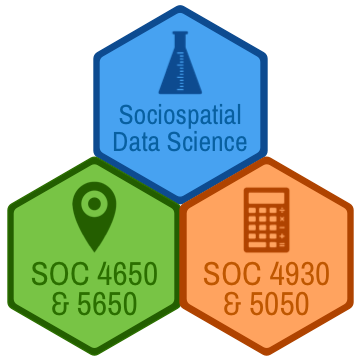
\includegraphics[width=0.4\linewidth]{images/SSDSBookBanner} \end{center}

This text is a companion text for both of my research methods courses at
\href{https://slu.edu}{Saint Louis University}:

\begin{itemize}
\tightlist
\item
  \href{https://slu-soc5650.github.io}{SOC 4650/5650 - Introduction to
  Geographic Information Science}
\item
  \href{https://slu-soc5050.github.io}{SOC 4930/5050 - Quantitative
  Analysis: Applied Inferential Statistics}
\end{itemize}

The goal of the text is to create a reference for the intangible, subtle
or disparate skills and ideas that contribute to being a successful
\emph{computational} social scientist. In writing this text, I draw
inspiration from the work of Donald Knuth.\footnote{\href{https://en.wikipedia.org/wiki/Donald_Knuth}{Donald
  Knuth} is the developer of
  \href{https://en.wikipedia.org/wiki/TeX}{TeX}, a computer typesetting
  system that is widely used today for scientific publishing in the form
  of \href{https://en.wikipedia.org/wiki/LaTeX}{LaTeX}. He also
  established the concept of
  \href{https://en.wikipedia.org/wiki/Literate_programming}{literate
  programming}, which forms the basis of some of the practices we follow
  with \texttt{R}.} Knuth has discussed his experiences in designing new
software languages, nothing that the developer of a new language

\begin{quote}
\ldots{}must not only be the implementer and the first large-scale user;
the designer should also write the first user manual\ldots{} If I had
not participated fully in all these activities, literally hundreds of
improvements would never have been made, because I would never have
thought of them or perceived why they were important\ldots{}
\end{quote}

While there is nothing particularly new about what I am writing here,
and I am certainly not developing a new language for computing, the goal
of this text remains similar to Knuth's experience. By distilling some
of key elements for making a successful transition to being a
\emph{professional developer} of knowledge rather than a \emph{casual
consumer}, I hope to both improve the course experience itself and also
create an environment that fosters a successful learning experience for
you.

In both classes, the course names are deceptive. We are not only
concerned with statistical work or mapping. Rather, we are more
fundamentally concerned with research methods. In particular, we are
concerned with \emph{high quality} research methods and the
\emph{process} of conducting research. We therefore focus on a
combination of mental habits and technical practices that make you a
successful researcher. Some of the skills and techniques that we will
discuss this semester are not taught as often in graduate programs, let
along undergraduate programs. Instead, they are often the products of
``learning the hard way''. These ``habits of mind and habits of method''
are broadly applicable across methodologies and disciplines.

\section*{License}\label{license}
\addcontentsline{toc}{section}{License}

Copyright © 2016-2018 \href{https://chris-prener.github.io}{Christopher
G. Prener}

This work is licensed under a Creative Commons Attribution 4.0
International License.

\chapter{Introduction}\label{intro}

The first part of this text is designed to help get you oriented to
coursework in computational social science. Both
\href{https://slu-soc5650.github.io}{Introduction to Geographic
Information Science (SOC 4650/5650)} and
\href{https://slu-soc5050.github.io}{Quantitative Analysis: Applied
Inferential Statistics (SOC 4930/5050)} are focused on building
students' capacities to address social science research questions using
tools that have been the traditional domain of computer and information
scientists. The growth and application of these tools in a variety of
disciplines both inside and outside of the social sciences has come to
be known as data science. Both courses are taught from this perspective,
so that while we focus on social science data, the tools and techniques
are broadly applicable across disciplines.

\section{What is data science?}\label{what-is-data-science}

Given data science's new emergence, its definition remains both
contested and often unclear. For me, there are four key aspects to focus
on when considering what constitutes data science:

\begin{enumerate}
\def\labelenumi{\arabic{enumi}.}
\tightlist
\item
  Statistics
\item
  Programming
\item
  Visualization and Communication
\item
  Substantive Knowledge
\end{enumerate}

I think of this as a ``full stack'' approach to computational research.
You want to be well versed not only the techniques for generating and
analyzing data, but also substantively in the academic literature about
your area of interest as well as ways to communicate your findings with
other researchers and the wider public.

\subsection{Statistics}\label{statistics}

Statistics covers the mathematical techniques that we use to draw
inference from our data. It is the main subject of one my courses,
\href{https://slu-soc5050.github.io}{Quantitative Analysis}. In
\href{https://slu-soc5650.github.io}{Introduction to GIS}, we do not
explicitly cover much in the way of inferential statistics. However, the
course is desinged to prepare you for a next level, Intermediate GIS
course that covers spatial statistics.

\subsection{Programming}\label{programming}

Computer programming is an essential part of data science broadly and
computational social science more specifically. Using a programming
language means that our work can be easily reproduced. This emphasis on
\textbf{reproducibility} is a response to a growing fear in many
disciplines that results are replicable from study to study, which
raises questions about the validity of much of the research work that we
do. Our goal in both courses is to produce research that is as
reproducible as possible.

This book introduces two programming languages -
\href{https://en.wikipedia.org/wiki/R_(programming_language)}{\texttt{R}}
and
\href{https://en.wikipedia.org/wiki/Python_(programming_language)}{Python}.
In \href{https://slu-soc5050.github.io}{Quantitative Analysis}, we will
be focused exclusively on learning \texttt{R} and using it to produce
statistical analyses. In
\href{https://slu-soc5650.github.io}{Introduction to GIS}, we will spend
a lot of time in \texttt{R}, but we will also use some Python to help
pass data from \texttt{R} to ArcGIS, the mapping application we will
use. I will also provide some additional Python lessons to folks who are
interested, but these will not be required for the course.

\subsection{Visualization \&
Communication}\label{visualization-communication}

Visualization is a fundamental aspect of data science work. It is how we
make our results easily digestible and accessible to a wider audience,
many of whom may not be able to interpret statistical output but can
learn from a well-designed scatter plot. In
\href{https://slu-soc5050.github.io}{Quantitative Analysis}, we will
focus on building plots to communicate information about statistical
distributions and the relationships between our variables. In
\href{https://slu-soc5650.github.io}{Introduction to GIS}, we will use
the same fundamental skills to build simple maps in \texttt{R}. We will
extend our emphasis on visualization to ArcGIS, where we will focus on
producing cartographically rich depictions of our data.

Separetely, we will discuss the presentation of statistical data in
tables using \href{https://en.wikipedia.org/wiki/LaTeX}{LaTex} in
\href{https://slu-soc5050.github.io}{Quantitative Analysis} as well as
the producing to conference-style presentations to communicate research
findings. In \href{https://slu-soc5650.github.io}{Introduction to GIS},
we will focus on producing conference-style posters instead. These are
different mediums, but they rely on the same design fundamentals that
are covered in this text.

\subsection{Substantive Knowledge}\label{substantive-knowledge}

Substantive knowledge covers two tangentially related topics: the
ability to work well in groups and the ability to digest and integrate
an academic literature into your own research. Each of these topics
receive some focus in both
\href{https://slu-soc5050.github.io}{Quantitative Analysis} and
\href{https://slu-soc5650.github.io}{Introduction to GIS}. Each class
has some group work associated with the completion with weekly lab
assignments. \href{https://slu-soc5650.github.io}{Introduction to GIS}
also has a group work component associated with the final project. In
each class, students' final projects are focused on a specific content
area that requires at least some background research and knowledge.
Synthesizing this knowledge and integrating it into your final projects
is a key piece of addressing this facet of data science.

\section{How is this book organized?}\label{how-is-this-book-organized}

Like many books about data science, this text follows a number of
standard conventions related to how it is organized and how examples are
given. This section introduces those conventions.

\subsection{Typefaces and Fonts}\label{typefaces-and-fonts}

Technical publications that describe scientific computing processes use
a \texttt{monospaced\ typewriter\ style\ typeface} to refer to commands
(inputs) and results (outputs). In some documents, like lecture slides
and cheat-sheets, I may highlight a command by using a particular color
to increase the visibility of the command name itself.

The \texttt{typewriter\ typeface} is also used to refer to functions
(e.g. \texttt{library()}), filenames (e.g. \texttt{mpg.csv}) or
filepaths (e.g.
\texttt{C:\textbackslash{}Users\textbackslash{}JSmith\textbackslash{}Desktop}).
Finally, we will use the \texttt{typewriter\ typeface} to refer to
GitHub repositories (e.g. \texttt{Core-Documents}, the repository that
contains this file).

Technical publications use \emph{italicized text} to refer to text that
is meant to be replaced. These references will typically appear in a
\texttt{typewriter\ typeface} since they are often part of commands. For
example, \texttt{str(dataFrame)} (with \texttt{dataFrame}
\emph{italicized}) indicates that you should replace the text
\texttt{dataFrame} with the appropriate variable name from your dataset.

These publications also use a sans serif typeface to refer to areas of
the user interface, menu items, and buttons. I cannot replicate that
here because of the publishing software that I use, but you'll notice
this text in course documents. We will therefore use the
\texttt{typewriter\ typeface} in the User Guide to identify these same
features.

Technical documents also use a sans serif or \texttt{typewriter}
typeface to refer to keyboard keys (e.g. \texttt{Crtl+C}) where the plus
sign (\texttt{+}) indicates that you should press multiple keys at the
same time. A sans serif typeface combined with a right facing
triangle-style arrow (\texttt{\textgreater{}}) is used to refer to
actions that require clicking through a hierarchy of menus or windows
(e.g. \texttt{File\ \textgreater{}\ Save}).

\subsection{Data}\label{data}

There are two sets of data that are used in this text, and they are also
used as part of \href{https://slu-soc5050.github.io}{Quantitative
Analysis} and \href{https://slu-soc5650.github.io}{Introduction to GIS}.
Both are available as \texttt{R} packages. The \texttt{testDriveR}
package contains some generic data that are particularly well suited for
exploring statistical topics. The \texttt{stlData} package contains data
that can be mapped at various levels. Both of these packages are
currently available on \href{https://github.com}{GitHub}, and can be
installed using the \texttt{devtools} package:

\begin{Shaded}
\begin{Highlighting}[]
\KeywordTok{install.packages}\NormalTok{(}\StringTok{"devtools"}\NormalTok{)}
\KeywordTok{library}\NormalTok{(devtools)}
\NormalTok{devtools}\OperatorTok{::}\KeywordTok{install_github}\NormalTok{(}\StringTok{"chris-prener/testDriveR"}\NormalTok{)}
\NormalTok{devtools}\OperatorTok{::}\KeywordTok{install_github}\NormalTok{(}\StringTok{"chris-prener/stlData"}\NormalTok{)}
\end{Highlighting}
\end{Shaded}

\subsection{Examples}\label{examples}

Throughout the semester, I will give you examples both in lecture slides
and in an example do-file. Examples in lectures and course documents can
be easily identified by their use of the \texttt{typewriter\ typeface}:

\begin{Shaded}
\begin{Highlighting}[]
\OperatorTok{>}\StringTok{ }\KeywordTok{library}\NormalTok{(stlData)}
\OperatorTok{>}\StringTok{ }\KeywordTok{str}\NormalTok{(stlLead)}
\StringTok{'data.frame'}\OperatorTok{:}\StringTok{   }\DecValTok{106}\NormalTok{ obs. of  }\DecValTok{15}\NormalTok{ variables}\OperatorTok{:}
\StringTok{ }\ErrorTok{$}\StringTok{ }\NormalTok{geoID         }\OperatorTok{:}\StringTok{ }\NormalTok{num  }\FloatTok{2.95e+10} \FloatTok{2.95e+10} \FloatTok{2.95e+10} \FloatTok{2.95e+10} \FloatTok{2.95e+10}\NormalTok{ ...}
 \OperatorTok{$}\StringTok{ }\NormalTok{tractCE       }\OperatorTok{:}\StringTok{ }\NormalTok{int  }\DecValTok{118100} \DecValTok{117400} \DecValTok{126700} \DecValTok{119102} \DecValTok{126800} \DecValTok{126900} \DecValTok{108100} \DecValTok{127000} \DecValTok{127400} \DecValTok{103700}\NormalTok{ ...}
 \OperatorTok{$}\StringTok{ }\NormalTok{nameLSAD      }\OperatorTok{:}\StringTok{ }\NormalTok{chr  }\StringTok{"Census Tract 1181"} \StringTok{"Census Tract 1174"} \StringTok{"Census Tract 1267"} \StringTok{"Census Tract 1191.02"}\NormalTok{ ...}
 \OperatorTok{$}\StringTok{ }\NormalTok{countTested   }\OperatorTok{:}\StringTok{ }\NormalTok{int  }\DecValTok{345} \DecValTok{871} \DecValTok{458} \DecValTok{182} \DecValTok{486} \DecValTok{1296} \DecValTok{903} \DecValTok{585} \DecValTok{2116} \DecValTok{417}\NormalTok{ ...}
 \OperatorTok{$}\StringTok{ }\NormalTok{pctElevated   }\OperatorTok{:}\StringTok{ }\NormalTok{num  }\FloatTok{9.57} \FloatTok{12.06} \FloatTok{18.12} \FloatTok{2.2} \FloatTok{4.73}\NormalTok{ ...}
 \OperatorTok{$}\StringTok{ }\NormalTok{totalPop      }\OperatorTok{:}\StringTok{ }\NormalTok{int  }\DecValTok{1161} \DecValTok{4307} \DecValTok{1089} \DecValTok{3237} \DecValTok{3490} \DecValTok{4590} \DecValTok{3144} \DecValTok{2052} \DecValTok{5486} \DecValTok{2408}\NormalTok{ ...}
 \OperatorTok{$}\StringTok{ }\NormalTok{totalPop_MOE  }\OperatorTok{:}\StringTok{ }\NormalTok{int  }\DecValTok{192} \DecValTok{447} \DecValTok{199} \DecValTok{309} \DecValTok{231} \DecValTok{826} \DecValTok{464} \DecValTok{273} \DecValTok{516} \DecValTok{274}\NormalTok{ ...}
 \OperatorTok{$}\StringTok{ }\NormalTok{white         }\OperatorTok{:}\StringTok{ }\NormalTok{int  }\DecValTok{414} \DecValTok{2604} \DecValTok{432} \DecValTok{2008} \DecValTok{3026} \DecValTok{148} \DecValTok{108} \DecValTok{304} \DecValTok{1777} \DecValTok{2149}\NormalTok{ ...}
 \OperatorTok{$}\StringTok{ }\NormalTok{white_MOE     }\OperatorTok{:}\StringTok{ }\NormalTok{int  }\DecValTok{100} \DecValTok{303} \DecValTok{116} \DecValTok{262} \DecValTok{270} \DecValTok{217} \DecValTok{111} \DecValTok{82} \DecValTok{391} \DecValTok{212}\NormalTok{ ...}
 \OperatorTok{$}\StringTok{ }\NormalTok{black         }\OperatorTok{:}\StringTok{ }\NormalTok{int  }\DecValTok{724} \DecValTok{1338} \DecValTok{631} \DecValTok{646} \DecValTok{194} \DecValTok{4320} \DecValTok{3020} \DecValTok{1739} \DecValTok{3603} \DecValTok{156}\NormalTok{ ...}
 \OperatorTok{$}\StringTok{ }\NormalTok{black_MOE     }\OperatorTok{:}\StringTok{ }\NormalTok{int  }\DecValTok{179} \DecValTok{374} \DecValTok{187} \DecValTok{210} \DecValTok{98} \DecValTok{760} \DecValTok{442} \DecValTok{283} \DecValTok{621} \DecValTok{190}\NormalTok{ ...}
 \OperatorTok{$}\StringTok{ }\NormalTok{povertyTot    }\OperatorTok{:}\StringTok{ }\NormalTok{int  }\DecValTok{324} \DecValTok{615} \DecValTok{506} \DecValTok{958} \DecValTok{349} \DecValTok{1743} \DecValTok{652} \DecValTok{331} \DecValTok{2524} \DecValTok{254}\NormalTok{ ...}
 \OperatorTok{$}\StringTok{ }\NormalTok{povertyTot_MOE}\OperatorTok{:}\StringTok{ }\NormalTok{int  }\DecValTok{140} \DecValTok{255} \DecValTok{164} \DecValTok{234} \DecValTok{129} \DecValTok{825} \DecValTok{305} \DecValTok{156} \DecValTok{598} \DecValTok{88}\NormalTok{ ...}
 \OperatorTok{$}\StringTok{ }\NormalTok{povertyU18    }\OperatorTok{:}\StringTok{ }\NormalTok{int  }\DecValTok{109} \DecValTok{169} \DecValTok{98} \DecValTok{15} \DecValTok{35} \DecValTok{627} \DecValTok{256} \DecValTok{47} \DecValTok{1110} \DecValTok{15}\NormalTok{ ...}
 \OperatorTok{$}\StringTok{ }\NormalTok{povertyU18_MOE}\OperatorTok{:}\StringTok{ }\NormalTok{int  }\DecValTok{105} \DecValTok{156} \DecValTok{60} \DecValTok{25} \DecValTok{47} \DecValTok{595} \DecValTok{136} \DecValTok{79} \DecValTok{318} \DecValTok{23}\NormalTok{ ...}
\end{Highlighting}
\end{Shaded}

Examples will almost always use the dataframe \texttt{stlLead}, which
comes with the \texttt{stlData} package. To open it, simply load the
\texttt{stlData} package using the \texttt{library()} function and then
start referencing \texttt{stlLead} anytime you need a dataframe. This
allows you to easily recreate examples by minimizing dependencies within
your code.

\part{First Steps}\label{part-first-steps}

\chapter{Approaching These Courses}\label{approaching-these-courses}

Students have varying experiences learning computational techniques. For
some, the math and programming that are the foundation for modern data
science techniques come naturally. For others, being introduced to these
concepts can be an anxiety producing experience. I am fond the phrase
``your mileage will vary'' for describing these differences - no two
students have the exact same experience taking a computational methods
course. Like the previous chapter, some of the content below is specific
to the courses (\href{https://slu-soc5650.github.io}{Introduction to
Geographic Information Science (SOC 4650/5650)} and
\href{https://slu-soc5050.github.io}{Quantitative Analysis: Applied
Inferential Statistics (SOC 4930/5050)}) I teach at
\href{https://www.slu.edu}{Saint Louis University}, the general outlook
on approaching data science work that I describe below is hopefully
applicable in a far wider arena.

\hypertarget{zen-and-the-art-of-data-analysis}{\section{Zen and the Art
of Data Analysis}\label{zen-and-the-art-of-data-analysis}}

One of the biggest challenges with this course can be controlling the
anxiety that comes along with learning new skills. \texttt{R} synatx,
GIS terms, LaTeX commands, and Markdown can seem like foreign alphabets
at first. Debugging \texttt{R} synatx can be both challenging and a
large time suck, in part because you are not yet fluent with this
language. Imagine trying to proofread a document written in a language
that you only know in a cursory way but where you must find minute
inconsistencies like misplaced commas.

For this reason, I also think it is worth reminding you that many
students in the social sciences struggle with computational methods at
first. It is normal to find this challenging and frustrating. I find
that students who can recognize when they are beginning to go around in
circles are often the most successful at managing the issues that will
certainly arise during this course. Recognizing the signs that you are
starting to spin your wheels and taking either ten minutes, an hour or
two, or a day away from computational coursework is often a much better
approach than trying to power through problems.

Data analysis therefore requires a certain mindfulness. I mentioned in
the \protect\hyperlink{preface}{Preface} that much of what this book
covers are ``habits of mind and habits of method''. These mental habits
extend past being able to recognize that frustration is setting in. They
also include the mental habits needed for
\protect\hyperlink{getting-and-staying-organized}{Getting and Staying
Organized} and strategies for \protect\hyperlink{getting-help}{Getting
Help} as you navigate the inevitable errors that come with learning new
analytical skills.

\hypertarget{getting-and-staying-organized}{\section{Getting and Staying
Organized}\label{getting-and-staying-organized}}

Doing data science work, and having the space to step away for a day as
the last section suggests, requires discipline and organization.
Similarly, computational coursework can demanding not just because it is
complex but because the courses often have a number of moving pieces
that you need to keep track of. Being mindful of this challenege from
the beginning, and taking steps to plan for it, is an important part of
this course.

\subsection{Keeping Track of Where You
Are}\label{keeping-track-of-where-you-are}

Students who have some system for tracking their work and creating to-do
lists are often the most successful in this course, not because they
have a fundamentally better grasp on the content but because they simply
are more organized. If you have never thought particularly hard about
how you manage tasks, now is an excellent time to start doing so. You do
not need fancy computer software to accomplish this, though there are an
array of possibilities if you do want to use software to keep yourself
organized. A legal pad or a notebook can be just as effective as a \$50
to-do list manager. The point is, do \emph{something}!

I am fond of recommending the
\href{http://gettingthingsdone.com}{\textbf{Getting Things Done}}
methodology to students as part of thinking more wholistically about
staying organized. The website \href{https://lifehacker.com}{Lifehacker}
posted an
\href{https://lifehacker.com/productivity-101-a-primer-to-the-getting-things-done-1551880955}{excellent
introduction to GTD} that is a great way to get a sense of how it works
and find additional resources for implementing it.

The GTD website has a
\href{http://gettingthingsdone.com/common-tools-software/}{great list of
software} for those of you looking for a to-do list application. One
that isn't listed that I use for collaborating with my student research
team is \href{https://trello.com}{Trello}, a freemium website that
allows you to create simple to-do lists. It isn't sophisticated enough
for implementing GTD, but it is more than sufficient for managing to-do
lists related to this course.

\subsection{Managing Course Materials}\label{managing-course-materials}

For both courses covered by this book, materials will be disseminated in
physical and digitial form. The topic of keeping digitial materials
organized is the subject of the next chapter. The physical handouts and
materials that we'll give out will all come three hole punched, and you
are expected to purchase a three-ring binder for this course. I give out
enough handouts that, without a binder, it becomes difficult to keep
track of where handouts are located. I have watched students spend more
time looking for the handout than it takes to find the answer to their
question once they have the handout itself.

There are two recommended ways to keep your binder tidy. One is to
organize by lecture. There are sixteen lectures worth of handouts in
both courses (not including the course preview and the final research
conference session), so two sets of dividers (which often come in packs
of eight) should be sufficient. The other way to organize handouts is by
topic. We hand out a number of different types of documents that could
be organized thematically like so:

\begin{enumerate}
\def\labelenumi{\arabic{enumi}.}
\tightlist
\item
  Syllabus and reading list
\item
  Workflow diagrams
\item
  \texttt{R} function sheets
\item
  ArcGIS process sheets (SOC 4650/5650 only)
\item
  LaTeX command sheets (SOC 4930/5050 only)
\item
  Sample outputs
\item
  Exercise handouts
\item
  Lab handouts
\item
  Problem set handouts
\end{enumerate}

Since there are approximately eight different types of handouts in each
class, a single package of dividers should be sufficient.

I don't think that one way of organization, thematically or temporally,
is inherently better or worse than the other. In large part it comes
down to how \emph{you} like to organize information. After all, learning
how to process and organize information in a way that works for you is
the most important takeaway here.

\section{Course Flow}\label{course-flow}

\begin{center}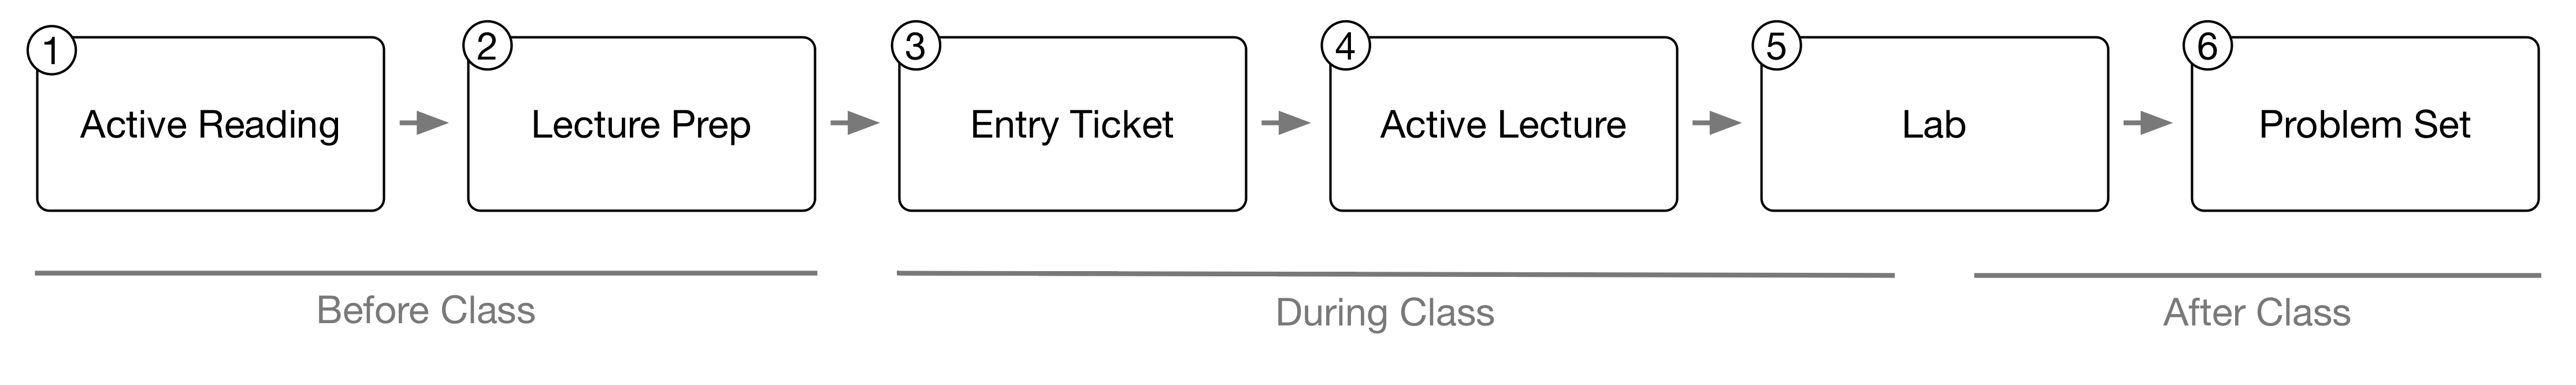
\includegraphics[width=1\linewidth]{images/courseWorkflow} \end{center}

Both \href{https://slu-soc5050.github.io}{Quantitative Analysis} and
\href{https://slu-soc5650.github.io}{Introduction to GIS} follow the
same weekly flow or progression. The structure of the assignments and
course materials presupposes that you adhere to this progression.

\subsection{Reading with Purpose}\label{reading-with-purpose}

The book and article \textbf{reading assignments} for this course are
different from most of the other reading you will do in your graduate
program because they are often very technical. Students who are most
successful in this course read twice. Read the first time to expose
yourself to the material, then take a break from the reading. During
this first read, I don't recommend trying to complete the example
problems or programming examples. Focus on the \emph{big picture} - what
are the concepts and ideas that these readings introduce?

During the second read, try to focus in in the \emph{details} - what are
the technical details behind the big picture concepts? I recommend doing
this second read with your computer open. Follow along with the examples
and execute as much of them as you can. By using this second read
through as a way to test the waters and experiment with the week's
content, you can come into the lecture better prepared to take full
advantage of the class period. Students who follow this approach are
able make important connections and focus on the essential details
during lectures because it is their third time being exposed to the
course material. They are also in a much stronger position to ask
questions.

\subsection{Lecture Preps}\label{lecture-preps}

Once you've completed the readings for the week, tackle the
\textbf{lecture prep}. These short assignments are designed to help
prepare you for the upcoming lecture by reviewing some of the concepts
from the reading. For many of the preps, I will post replication videos
on YouTube that show how to solve each problem and provide some
explanation for that process. Use this as an early indication of how
well you understood the readings and what questions you might have.
Bringing these questions to class is a great way to build your knowledge
of the course material.

\subsection{Active Lectures and Labs}\label{active-lectures-and-labs}

During \textbf{lectures}, I introduce many of the same topics that your
readings cover. This again is intentional - it gives you yet another
exposure to concepts and techniques that are central to geospatial
science. One mistake students sometimes make is focusing on the details
of \emph{how} to do a particular task rather than focusing on
\emph{when} a task should be done. If you know when a task is needed but
cannot remember how to do it in \texttt{R}, you can look this
information up. Conversely, detailed notes on executing \texttt{R}
commands may not be helpful if you are unsure when to use a particular
skill. There is no penalty in this course for not knowing how to execute
a command from memory; this is what reference materials are for. The
most successful students will therefore focus on \emph{when} a
particular skill is warranted first before focusing on \emph{how} to
execute that skill

Getting experience with executing tasks is the purpose of the
\textbf{lab exercises}. These are narrlowly defined and focused on
building your confidence with the specific skills introduced each week.
Time for beginning these exercises is given at the end of each class
meeting, and replication files will be posted on GitHub for each lab. I
suggest that students do not look at replication files until they are
truly stumped. Spend some time wrestling with problems and code, and
experiment with the trouble shooting process, when the stakes are low
and you have a saftey-net to catch you. This will prepare you to respond
to issues on the problem sets in a more resiliant way.

\subsection{Problem Sets}\label{problem-sets}

The problem sets are the key evaluation of your progress in the course.
These will cover skills both for the week they are assigned as well as
previous weeks to ensure that you are connecting various aspects of the
course and are able to transition skills from one week to the next.
Replication files will be provided after all problem sets are submitted
and grades are returned. Review these replication files regardless of
how well you do on a given problem set - there is much to learn from
reviewing your progress and seeing a different approach to these
assignments.

\subsection{An Apple a Day}\label{an-apple-a-day}

As I noted above, some degree of frustration with these courses is to be
expected - funtions in \texttt{R} will not work as intended, for
example, and the ambiguity of error messages can be excruicating. I
suggested above that you build into your approach to the course time to
walk away from assignments if you hit a wall. Being able to walk away
from an assignment for a day requires excellent time management. If you
are waiting until the night before or the day of an assignment's due day
to begin it, you give yourself little room for errors.

I recommend approaching this course in bite size chunks - a little each
day. The most successful students do not do all of their reading,
homework, and studying in a single sitting. I find that this approach
not only creates unnecessary anxiety around assignments, it also
dramatically limits the amount of course material you can absorb. Keep
in mind that I expect the \emph{median} student to spend approximately
six hours on work for this class each week (twice the amount of in-class
time). A sample approach to the class might look something like this:

\begin{itemize}
\tightlist
\item
  Monday: class
\item
  Tuesday: finish lab
\item
  Wednesday: Start problem set
\item
  Thursday: Finish problem set
\item
  Friday: First reading
\item
  Saturday: Second reading
\item
  Sunday: Lecture prep for next class
\end{itemize}

The single biggest failure point in both courses for students is
thinking that the few hours before class are sufficient for doing
\emph{all} of the work required for a particular week. It is the rare
student who can do this successfully (not only in terms of meeting the
required deadlines but also in terms of actually learning the material).
Err on the side of giving yourself too much time to complete work rather
than just enough!

\section{Staying Current}\label{staying-current}

Course content is maintained both on the respective course websites
(\href{https://slu-soc5050.github.io}{Quantitative Analysis} and
\href{https://slu-soc5650.github.io}{GIS}) and GitHub organizations
(\href{https://github.com/slu-soc5050}{Quantitative Analysis} and
\href{https://github.com/slu-soc5650}{GIS}). Course materials are
available throughout the semester and after the course is done. This
creates two challenges. First, for all students, attention must be paid
to when updates are pushed to GitHub and the course website. This is
particularly true for content updated \emph{after} a lecture. Second,
for students who like to work ahead, care must be taken to ensure that
you are working off of materials for the current semester and not the
last semester the course was taught. There are two ways in which I help
communicate the status of course content - badges and Slack.

\subsection{Badges}\label{badges}

I use badges on both the GitHub \texttt{README.md} files in individual
lecture repositories and on individual lecture webpages to signal which
semester the content is current for and what stage of development the
content is in. These badges are used not just because they are effective
but as part of a more general socialization into data science software
development, where badges are used to signal development status on
\texttt{R} package GitHub repositories. For example, the
\href{https://github.com/tidyverse/ggplot2}{\texttt{ggplot2}}
\texttt{README.md} file looks like this:

\begin{center}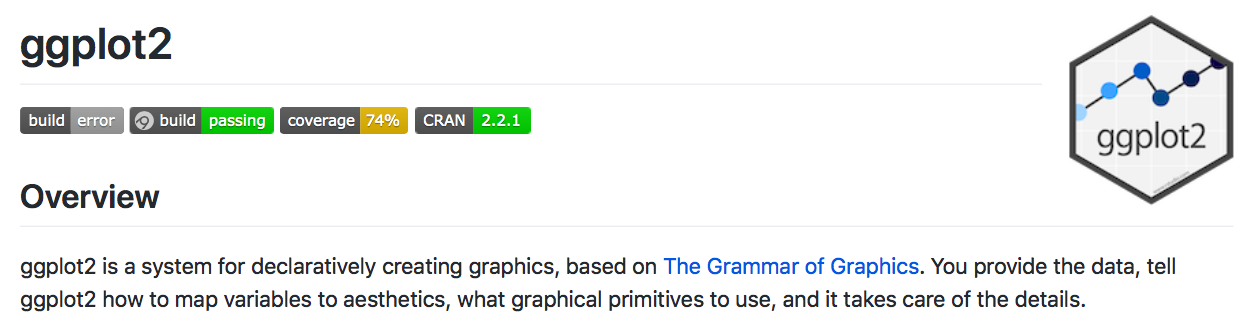
\includegraphics[width=0.95\linewidth]{images/ggplot2Readme} \end{center}

We can see from the first two badges that
\href{https://en.wikipedia.org/wiki/Continuous_integration}{continuous
integration services} are used, and that \texttt{ggplot2} is only
passing its tests on one of them. The third badge indicates that the
built-in tests of \texttt{ggplot2} test 74\% of the package's code. We
can also see from the fourth badge that the current version of the
software on CRAN is version 2.2.1 (as of December, 2017). Details like
this are not critical when you are first learning to use \texttt{R}, but
they grow more important as your data science skills progress.

We use the following badges for our course repositories and on the
course websites:

\begin{center}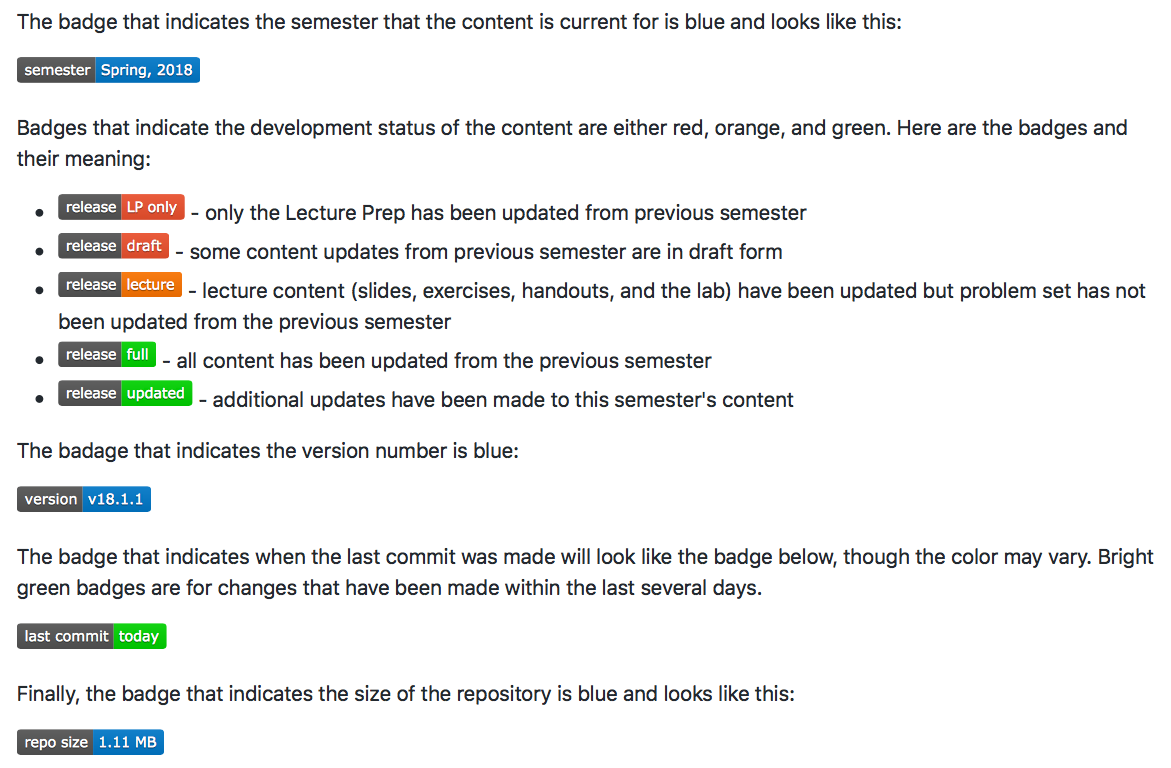
\includegraphics[width=0.95\linewidth]{images/readmeBadges} \end{center}

Here is an example of how the badges look on a course repository. As of
December 2017, the \texttt{README.md} associated with the
\href{https://github.com/slu-soc5050/Core-Documents}{\texttt{Core-Documents}
repository} for \href{https://slu-soc5050.github.io}{Quantitative
Analysis} looked like this:

\begin{center}
\includegraphics[width=0.95\linewidth]{images/readmeBadgesEx} \end{center}

We can see from the \texttt{README.md} that the contents are current for
the Fall 2017 semester from the first badge. The second badge indicates
that the contents have been updated since they were first released to
students. Finally, we can also see that the last commit was made today
(the day this screenshot was taken).

Here is an example of how the badges look on a course website. As of
December 2017, the
\href{https://slu-soc5650.github.io/course-preview}{Course Preview page}
for \href{https://slu-soc5650.github.io/}{GIS} looked like this:

\begin{center}
\includegraphics[width=0.95\linewidth]{images/webpageBadgesEx} \end{center}

From these two badges, we can see that the webpage is current for the
Spring 2018 semester and that it is the full release - no updates
additional are planned before the content is covered by students.

\subsection{Slack}\label{slack}

The \texttt{\#\_news} channel in each course's Slack organization will
be automatically updated with a list of commit messages for each lecture
repository. The updates will look like this:

\begin{center}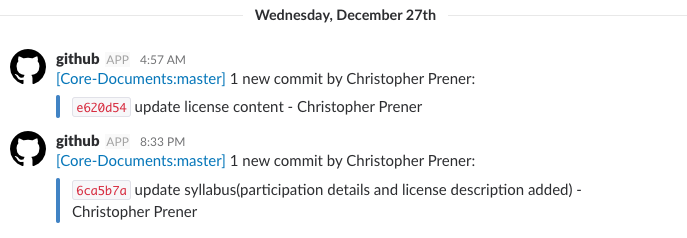
\includegraphics[width=0.95\linewidth]{images/slackNews} \end{center}

You will be able to scan through commit messages for updates that might
be relevant for you. From these messages, we can see that changes were
made to the \texttt{LICENSE} (one of the meta documents) in the
\href{https://github.com/slu-soc5650/Core-Documents}{\texttt{Core-Documents}
repository} for \href{https://slu-soc5650.github.io/}{GIS}. We can also
see that a change was made to the Syllabus's content for the course.

I recommend scanning through all new messages in \texttt{\#\_news} each
time you check in with the course on Slack. If you see changes, sync
your repository (if you are keeping local copies) or download the
updated document.

\chapter{Protecting Your Work}\label{protecting-your-work}

I believe that one of the biggest challenges to with doing computational
work is that it requires a high degree of organization. Prior to one of
my courses, students' approaches to file management on their computers
are often haphazard. I am very used to seeing students' desktops or
documents directories in various states of disarray. Perhaps that has
worked for them in the past, but that approach (or lack thereof)
\textbf{will} fail students in
\href{https://slu-soc5650.github.io}{Introduction to Geographic
Information Science (SOC 4650/5650)} and
\href{https://slu-soc5050.github.io}{Quantitative Analysis: Applied
Inferential Statistics (SOC 4930/5050)}. Moreover, if left un-checked,
it will fail students down the road when a hard drive failure or natural
disaster renders their data irrevocably inaccessible. This chapter
covers what some of those threats are and ways to manage those risks
when conducting computational research.

\section{Threats To Our Data}\label{threats-to-our-data}

Each semester that I teach
\href{https://slu-soc5650.github.io}{Introduction to GIS} and
\href{https://slu-soc5050.github.io}{Quantitative Analysis}, several
things happen. The first thing that happens is that students regularly
lose files. The effects of losing files can range from being a minor
frustration to a major headache depending on the file in question.
Losing files often results in downloading multiple copies of the same
data and recreating work. Both of these are wastes of your time.
Moreover, files are rarely gone. They are typically just misplaced. This
is bad for reproducibility, particularly when you happen across multiple
versions of the same file and have to sort out which version is the
version you last worked on.

The second thing that happens is that students who use thumb drives for
data storage lose them. Depending on the timing of this loss, this can
again range from being a minor frustration (very early in the semester)
to being downright anxiety attack producing (last few weeks of the
semester). Recreating an entire semester's worth of work on the final
project is both a tremendous waste of your time and a particularly
unpleasant experience.

Fortunately, I have never had a student's computer hard drive die during
the course of the semester. However, I assume that if I teach this
course long enough a hard drive failure will indeed occur. The backup
provider \href{https://www.backblaze.com/}{Backblaze} has
\href{https://www.backblaze.com/blog/how-long-do-disk-drives-last/}{analyzed}
their own hard drives and found that about 5\% of drives fail within the
first year. After four years, a quarter (25\%) of drives in their data
center fail.

Similarly, it is only a matter of time before a student's computer is
stolen along with all of their hard work. A less likely though still
very plausible scenario involves the destruction of a student's
belongings (computer and thumb drive included) in a fire, car accident,
or natural disaster.

Despite the likelihood that you will at some-point lose a thumb drive
(if not during this semester than sometime down the road) and the near
certainty that your computer's hard drive will eventually fail if a
rogue wave does not get it first, few students and faculty take these
risks seriously. While you cannot prevent many of these things from
happening, I want to suggest to you that you can take some simple steps
to sure that \emph{when} (not if) they happen, you are well prepared to
get back to work with minimal disruption.

\section{Data Management}\label{data-management}

One of the themes in \href{https://arxiv.org/abs/1609.00037}{``Good
Enough Practices in Scientific Computing''}, referenced in the previous
chapter, is an emphasis on data management. One of their core messages
is to ``save the raw data''. Particularly in GISc work, the raw data can
be expansive - dozens of shapefiles, tabular files, and associated
metadata. These files often come from disparate sources - city open data
sites, the U.S. Census Bureau, state data repositories, and other
federal agencies. Moreover, GIS data are often updated over time to
reflect on-the-ground changes. Saving the raw data in GISc work
therefore means not only creating a well-organized directory containing
\emph{all} of your original data. It also means logging the source of
each file, when it was downloaded, and (if applicable) a permanent web
link to your data source. For that reason, we'll give you not just the
course data but a read me file and a metadictionary that lists all of
the files we've disseminated to you.

A second message in the paper is to ``create the data you wish to see in
the world''. The authors encourage readers to ``create the dataset you
wish you had received.'' First and foremost, this means using open and
not proprietary data formats. For spatial data,
\href{https://en.wikipedia.org/wiki/Shapefile}{ESRI shapefiles} are
technically proprietary, though their standard is open. This means that
other software applications, like \texttt{R} and QGIS can read and in
some cases write shapefiles. For sharing spatial data, a better option
is the \href{https://en.wikipedia.org/wiki/GeoJSON}{GeoJSON}, which is a
plain text file format.

Tabular data are best stored as \texttt{CSV} files, which is also a
plain text file format that can be opened by a wide variety of
applications. In contrast, common file formats like Microsoft Excels's
\texttt{XLS} and \texttt{XLSX} are proprietary file packages that cannot
be read as plain text and are therefore less desirable for storing data.

\section{Creating a Sustainable File
System}\label{creating-a-sustainable-file-system}

In his excellent document \href{http://plain-text.co}{\emph{The Plain
Person's Guide to Plain Text Social Science}}, Kieran Healy describes
two important revolutions in computing that are currently taking place.
One of them is the advent of mobile touch-screen devices, which he notes

\begin{quote}
hide from the user both the workings of the operating system and
(especially) the structure of the file system where items are stored and
moved around.
\end{quote}

For most users, I would argue that this extends to their laptop or
desktop computers as well. I would venture to guess that the majority of
my students are used to keeping large numbers of files on their desktops
or in an (distressingly) disorganized \texttt{Documents} folder. For
research, particularly quantitative research, such an approach to file
management is unsustainable. It is difficult to produce \emph{any}
research, let alone work that is reproducible, without an active and
mindful approach to file management.

\subsection{\texorpdfstring{Create a \emph{Single} Course
Directory}{Create a Single Course Directory}}\label{create-a-single-course-directory}

The most successful approach to organizing files is to identify
\emph{one and only one} area that you will store course files in. Having
files scattered around you hard drive between you \texttt{Desktop}
directory, \texttt{Downloads}, \texttt{Documents}, and a half dozen
other places is a recipe for lost files. It can also add complexity to
the task of backing these files up. I recommend naming this directory
simply based on the course you are enrolled in:

\begin{itemize}
\tightlist
\item
  \texttt{SOC4650}
\item
  \texttt{SOC4930}
\item
  \texttt{SOC5050}
\item
  \texttt{SOC5650}
\end{itemize}

These names are short, have no punctuation or spaces (which can create
conflicts with software), and explicitly connects the directory to this
course as opposed to other courses you may take that are also statistics
or GIS courses (a good reason to avoid naming the directory
\texttt{Stats} or \texttt{GIS}!).

This single course directory should reside in \emph{one and only one}
place. Storing it inside a sync'd directory (like Dropbox or Google
Drive) may cause conflicts with your Git repositories. I strongly
recommend storing your course directory on the computer that you will
regularly do work on for the course. For some students, that will be the
desktop computer in our lab. For others, it will their laptop computer.
If you find yourself having to regularly switch between computers, I'll
provide some suggestions later in this chapter.

\subsection{Approach Organizing
Systematically}\label{approach-organizing-systematically}

Within your single course directory, I recommend following a mindful,
purposeful approach to organization. This approach begins with having a
number of dedicated subfolders within your course directory:

\begin{verbatim}
/SOC5650
  /Core-Documents
  /Data
  /DoeAssignments
  /FinalProject
  /Labs
  /Lectures
  /Notes
  /ProblemSets
  /Readings
  /WeeklyPreps
  /WeeklyRepos
\end{verbatim}

Note again how these directories are named - there are no spaces,
special characters, and the names are deliberately short but specific.
For a directory with two words (\texttt{FinalProject} or
\texttt{ProblemSets}), I use what is known as camelCase to name the file
where the second (any any subsequent) words have their first character
capitalized. You could also use dash-case (\texttt{Core-Documents}) or
snake\_case (\texttt{Core\_Documents}) as a naming strategy. Regardless
of which of these approaches you take, try to use it consistently.

Once you have these folders set-up, I want you to an agreement with
yourself: files for the course will \emph{only} be saved within this
structure. Do not temporarily save files to the \texttt{Desktop}, for
example, intending to move them later. They will be forgotten.

\subsection{\texorpdfstring{The \texttt{Core-Documents}
Directory}{The Core-Documents Directory}}\label{the-core-documents-directory}

This directory has already been created and will be added to your file
system during \textbf{Week 03}, when it is \textbf{cloned} from GitHub.

\begin{rmdnote}
A cloned directory is one that retains a digital link to the data stored
on GitHub, meaning that it can be easily updated if changes are made.
This will be explained in greater depth in Introduction to GitHub
chapter in this text.
\end{rmdnote}

\begin{rmdwarning}
You will not be able to push changes that you make in this directory to
GitHub, and making other changes could cause conflicts. I suggest not
making changes inside this repository beyond opening files for reference
purposes.
\end{rmdwarning}

The \texttt{Core-Documents} directory is used for storing the course
syllabus, reading list, and a sample schedule for 3600 Morrissey Hall
for the semester.

\subsection{\texorpdfstring{The \texttt{Data}
Directory}{The Data Directory}}\label{the-data-directory}

\begin{rmdwarning}
This directory is only applicable to students in
\href{https://slu-soc5650.github.io}{Introduction to GIS}, who will
receive a data release at the beginning of the semester that should be
saved here. Students in
\href{https://slu-soc5050.github.io}{Quantitative Analysis} will receive
most data through \texttt{R} packages and may reiceve a small amount of
data through weekly repositories.
\end{rmdwarning}

The data directory should have copies of any original data and their
documentation that are not disseminated to you as \texttt{R} packages.
Most of these data are included in the initial data release, but you
will have to add some additional data to this directory over the course
of the semester. The data in this directory should be used as needed but
not altered (one of the of the ``good enough'' research practices from
the previous chapter).

\subsection{\texorpdfstring{The \texttt{DoeAssignments}
Directory}{The DoeAssignments Directory}}\label{the-doeassignments-directory}

Like the \texttt{Core-Documents} repository, this will not be included
in the course data release. You will add it to your file system during
\textbf{Lab-03}. It will also have a different name - your last name
instead of `Doe'. Once you add it, it will contain a number of
subdirectories:

\begin{verbatim}
  /SOC5650
    /DoeAssignments
      /FinalProject
        /Documentation
        /Memo
        /PaperDraft
        /PaperFinal
        /PosterDraft
        /PosterFinal

      /Labs
        /Lab-01
        ...
        /Lab-16

      /ProblemSets
        /PS-01
        ...
        /PS-10
      
      /WeeklyPrep
        /WP-02
        ...
        /WP-16
\end{verbatim}

The \texttt{FinalProject} directory contains submission folders for each
component of the final project. If you a registered for SOC 4650, your
directory will look like what appears above. Students registered for SOC
5650 will have three additional subfolders for deliverables related to
the final paper element of the course.

The \texttt{Labs}, \texttt{ProblemSets}, \texttt{WeeklyPrep} directories
have subfolders dedicated to the individual assignments you'll have to
submit over the course of the semester. \textbf{These directories are
intended to store only the deliverables that are requested in each
assignment's directions.} All other files related to each assignment
should be stored elsewhere in your folder structure.

\begin{rmdwarning}
Unlike \texttt{Core-Documents}, you have the ability to push changes
made here to GitHub.com. Please make sure you understand that changes
made will be reflected, for better or worse, on the website the next
time you complete that push.
\end{rmdwarning}

\subsection{\texorpdfstring{The \texttt{FinalProject}
Directory}{The FinalProject Directory}}\label{the-finalproject-directory}

The final project directory should be a microcosm of the larger
directory structure, with most major directories replicated so that your
final project files have a dedicated, organized home:

\begin{verbatim}
  /SOC5650
    /FinalProject
      /AnnotatedBib
      /Data
      /DataAnalysis
      /Documentation
      /Memo
      /Notes
      /Paper
      /Poster
      /Readings
\end{verbatim}

You'll notice that there are a number of new directories dedicated to
specific aspects of the project.

\begin{rmdnote}
You will want to tailor this subdirectory's contents to match the
specific requirements of the section you are enrolled in. This may
entail removing certain folders - the \texttt{AnnotatedBib/} for example
- that do not correspond to deliverables you have to complete.
\end{rmdnote}

\subsection{\texorpdfstring{The \texttt{Labs}, \texttt{ProblemSets}, and
\texttt{WeeklyPreps}
Directories}{The Labs, ProblemSets, and WeeklyPreps Directories}}\label{the-labs-problemsets-and-weeklypreps-directories}

This directory contains subfolders for each of the sixteen lab
assignments for this course. Save \emph{all} of the associated materials
for each lab assignment here.

\begin{verbatim}
  /SOC5650
    /Labs
      /Lab-01
      ...
      /Lab-16
      
    /ProblemSets
      /PS-01
      ...
      /PS-10
      
    /WeeklyPreps
      /Week-01
      ...
      /Week-16
\end{verbatim}

These directories differ from what you save in your
\texttt{DoeAssignments} repository. Unlike \texttt{DoeAssignments},
which is \textbf{only} for submission files, these directories can
contain any number of files you wish. Use each of these assignment
folders as a place to work and experiment, and the folders under
\texttt{DoeAssignments} as the place to submit your final versions.

Each of these assignments that utilizes \texttt{R} and RStudio should
have an R Project associated with it:

\begin{verbatim}
  /SOC5650
    /Labs
      /Lab-01
        Lab-01.Rproj
        
      /Lab-02
        Lab-02.Rproj
        
      /Lab-03
        Lab-03.Rproj
\end{verbatim}

Using R Projects will help you keep your work organized by ensuring that
the working directory for RStudio is correctly set every time and that
output is always saved to the appropriate assignment directory.

\subsection{\texorpdfstring{The \texttt{Lectures}
Directory}{The Lectures Directory}}\label{the-lectures-directory}

This directory should contain subfolders for each of the sixteen weeks
of the course. When we create new files during lectures, save these
documents in the appropriate week's folder.

\begin{verbatim}
  /SOC5650
    /Lectures
      /Week-01
      ...
      /Week-16
\end{verbatim}

\subsection{\texorpdfstring{The \texttt{Notes}
Directory}{The Notes Directory}}\label{the-notes-directory}

Use this as a home for course notes if you decide to take notes
digitally and do not already use notebook software of some kind that
organizes notes for you.

\subsection{\texorpdfstring{The \texttt{Readings}
Directory}{The Readings Directory}}\label{the-readings-directory}

Use this as a home for \texttt{.pdf} copies of course readings. I
suggest creating subdirectories \emph{only} for weeks that have readings
assigned from outside of the main texts, such as Week 01:

\begin{verbatim}
  /SOC5650
    /Readings
      /Week-01
\end{verbatim}

\subsection{\texorpdfstring{The \texttt{WeeklyRepos}
Directory}{The WeeklyRepos Directory}}\label{the-weeklyrepos-directory}

Clone each of the weekly repos to this directory, and sync them when
updates are made to ensure you have the latest versions of files. By the
end of the course, this directory should have sixteen subfolders like
this:

\begin{verbatim}
  /SOC5650
    /WeeklyRepos
      /Week-01
      ...
      /Week-16
\end{verbatim}

\begin{rmdwarning}
You will not be able to push changes that you make in these directories
to GitHub, and making other changes could cause conflicts. I suggest not
making changes inside this repository beyond opening files for reference
purposes. If there is something you need to edit, copy it to the
appropriate subdirectory (\texttt{Labs}, \texttt{WeeklyPreps}, etc.) and
make local changes there.
\end{rmdwarning}

\section{Backing Up Your Data}\label{backing-up-your-data}

There are a number of different ways to think about backing up your
data. The most successful backup strategies will incorporate all of
these elements.

\subsection{Bootable Backups}\label{bootable-backups}

``Bootable'' backups are mirrored images of your \emph{entire} hard
drive, down to temporary files, icons, and system files. With a bootable
backup, you can restore your entire computer in the event of a hard
drive failure or a corruption of the operating system files. They are
named as such because you can plug in the external drive that you are
using for this backup and literally boot your computer up from that
drive (typically a \emph{very} slow process).

These backups are often made less frequently because they can be
resource intensive and it is best not to use your operating system while
creating a clone. They are typically made to an external hard drive,
which is subject to similar failure rates as the hard drives inside your
computer. So bootable drives need to be replaced every few years to
maintain their reliability.

Both major operating systems come with applications for creating clones
of your main hard drive that are bootable, and there are a number of
third party applications that provide this service as well.

\subsection{Incremental Backups}\label{incremental-backups}

Incremental backups are designed to keep multiple copies of a single
file (how often depends on the type of software you use and the settings
you select). These can be used to restore an older copy of a file if
work is lost or a newer file is corrupted.

Apple's TimeMachine is a great example of an incremental backup - when
kept on, it creates hourly backups of files that have been changed,
daily backups for the previous month, and weekly backups for previous
months. Once the disk is full, the oldest backups are deleted. Dropbox
also provides a similar service, retaining all previous versions of
files (and deleted files) for thirty days.

Incremental backups are typically good options for recovering files that
have been recently changed (again, depending on the software you use and
the settings you select). Since they run frequently (every time a file
is changed or every hour, for example), recent changes tend to get
captured. They can be limited in terms of their long-term storage - it
may not be possible to recover older versions of a file past a few
weeks.

They are also not always good solutions for recreating your entire
computer since they do not save all necessary program and operating
system files, and may be cumbersome to work with if you need to recover
a large quantity of files. Like bootable backups, these are typically
stored on external hard drives that need to be replaced on a regular
basis.

In addition to the aforementioned Apple TimeMachine, the Windows OS also
comes with a built-in service for creating incremental backups. Dropbox
is a good option if you have a small number of files, but you may find
the need to upgrade to a paid account if you have a large amount of
data.

\subsection{Cloud Backups}\label{cloud-backups}

Cloud backup services like \href{https://www.backblaze.com}{Backblaze}
or \href{https://www.code42.com/crashplan/}{Crashplan} offer
comprehensive backup solutions for customers. These plans typically
require a monthly subscription fee to maintain access to your backups.
While bootable backups protect against hard drive failure and
incremental backups protect against data corruption, cloud backups
protect against catastrophic events like robberies, fires, and other
natural disasters. A fire or a tornado that affect your house may
destroy your laptop and any external hard drives you use for backup, but
your cloud backup will be unaffected.

\subsection{A Workflow for Backups}\label{a-workflow-for-backups}

Just as we need a workflow for approaching file management, it is also
important to establish a routine for backups. With backups, the most
successful workflows are those that require next to no effort on your
part. If you primarily use a desktop, this can be as simple as leaving
two external hard drives plugged into your computer since most backup
software can be set to run automatically. If you have tasks that require
you to manually do something (plug an external hard drive into your
computer, for instance), create a reminder for yourself on a paper
calendar or a digital calendar or to-do list application.

\begin{rmdtip}
I gave a presentation on workflows for backing data up as part of the
\href{https://slu-dss.github.io}{Data Science Seminar} series at
\href{https://slu.edu}{Saint Louis University}. You can easily view the
slides from that presentation on
\href{https://speakerdeck.com/chrisprener/protecting-your-data}{Speaker
Deck}, and you can download the session's materials from
\href{https://github.com/slu-dss/protectData}{GitHub}.
\end{rmdtip}

For this course in particular, it is \emph{imperative} that you backup
the data on your flash drive. A number of possibilities exist for
accomplishing this:

\begin{itemize}
\tightlist
\item
  Keep a local copy of your flash drive's files on your computer.
\item
  Keep a \texttt{.zip} archive of your files in a service like Dropbox
  or Google Drive. (Using a \texttt{.zip} archive will prevent issues
  with your \texttt{.git} repositories.)
\item
  Maintain a second flash drive copies of all of your files.
\end{itemize}

Whatever solution you select, make sure you regularly update your
backup. The more often you keep your backup archive updated, the less
stressful and disruptive losing your drive will be. This will likely be
a manual task, so follow the guidance above about creating a repeating
calendar event or to-do list task reminder.

\section{Managing Multiple Devices}\label{managing-multiple-devices}

If you are trying to manage your work across multiple computers, the
task of staying organized becomes more difficult. One option is to use a
thumb drive or external hard drive as the primary site where your course
directory lives. That way you can save everything there and it is
accessible by as many computers as necessary. If you decide go this
route, it is \textbf{imperative} that you back-up your work to a
computer or to another external drive.

\begin{rmdtip}
macOS users should make sure that the external drive is formatted using
the ExFat file system specification so that it is readable both by their
operating system and the Windows operating system in the computer lab.
If you buy a new drive, you will likely have to re-format it.
\end{rmdtip}

Another option is to utilize GitHub extensively. You can create repos
for the some of the key subdirectories referenced above, like
\texttt{ProblemSets}, \texttt{WeeklyPreps}, and others, and keep you
work synced between computers using the same process we use for
submitting work. If you want to do this, make sure you get the
\href{https://education.github.com/discount_requests/new}{student GitHub
discount}, which will give you unlimited private repositories. That way,
your course work will not be public facing. If you pursue this strategy,
make sure you still have only one place for a specific file typoe - you
do not want some problem set materials saved outside of your GitHub repo
and some saved in it.

\chapter{\texorpdfstring{``Good Enough'' Research
Practices}{Good Enough Research Practices}}\label{good-enough-research-practices}

This section introduces some of the core concepts that we will emphasize
in this course throughout the semester. The title takes inspiration from
a recent article titled \href{https://arxiv.org/abs/1609.00037}{``Good
Enough Practices in Scientific Computing''}\footnote{Wilson, G., Bryan,
  J., Cranston, K., Kitzes, J., Nederbragt, L. and Teal, T.K., 2016.
  Good Enough Practices in Scientific Computing. \emph{arXiv preprint
  arXiv:1609.00037.}}. The authors note in their introduction that
scientific computing advice can sometimes be both overwhelming and
focused on tools that are inaccessible to many analysts. Their goal, and
the goal of this course, is to de-mystify the simplist tools that enable
researchers to streamline their workflows:

\begin{quote}
Our intended audience is researchers who are working alone or with a
handful of collaborators on projects lasting a few days to a few months,
and who are ready to move beyond emailing themselves a spreadsheet named
\texttt{results-updated-3-revised.xlsx} at the end of the
workday\ldots{}Many of our recommendations are for the benefit of the
collaborator every researcher cares about most: their future self.
\end{quote}

I would argue that the skills they describe are useful beyond just a few
months. Indeed, most of the skills here can dramatically improve
students' dissertation experiences:

\begin{quote}
Most importantly, these practices make researchers more productive
individually by enabling them to get more done in less time and with
less pain. They also accelerate research as a whole by making
computational work (which increasingly means all work) more
reproducible. But progress will not happen by itself. Universities and
funding agencies need to support training for researchers in the use of
these tools. Such investment will improve confidence in the results of
computational work and allow us to make more rapid progress on important
research questions.
\end{quote}

While much of what we will talk about in this course is aimed at
supporting your work, there are benefits that extend beyond your
dissertation or your research projects. These benefits, which include
developing sustainable workflows and structuring the way you interact
with your own computer, can make everyday computing practices like
checking email or organizing files an easier, more structured process.

\section{Reproducibility}\label{reproducibility}

One of the mantras of this course is our emphasis on reproducibility.
The unifying feature of all of the ``good enough'' research practices
discussed below is that they contribute to a more reproducible research
product.

Reproducibility is very much in vogue right now for number of reasons.
\href{http://science.sciencemag.org/content/349/6251/aac4716}{Assessments
of studies in psychology}\footnote{Open Science Collaboration, 2015.
  Estimating the reproducibility of psychological science.
  \emph{Science}, 349(6251), p.aac4716.}, for example, have found weaker
on average effect sizes and far fewer statistically significant results
than the initial studies reported. There have also been high profile
instances of falsified research, including
\href{http://nymag.com/scienceofus/2015/05/how-a-grad-student-uncovered-a-huge-fraud.html}{research
by a graduate student at UCLA}. This particular instance of fraud was
identified by graduate students intent on replicating the original
study.

At the same time, there is a recognition that the skills necessary for
producing reproducible research are not being fostered in academic
disciplines and graduate programs. Thus one of the goals of this course,
and this \textbf{User's Guide} in particular, is to help develop a
working knowledge of many of these skills.

One challenge, however, is that reproducibility does not have a
consistent definition. Some researchers use the term to narrowly refer
to code that can execute without alteration on a person's computer.
Others use it to refer to research designs that can be replicated by
other researchers. Still others discuss reproducibility as the ability
to obtain a similar set of results or draw similar inferences from
identical research designs.

When we talk about reproducibility in this class. We'll be primarily
concerned with \textbf{methods reproducibility}:

\begin{quote}
the ability to implement, as exactly as possible, the experimental and
computational procedures, with the same data and tools, to obtain the
same results.\footnote{Goodman, S.N., Fanelli, D. and Ioannidis, J.P.,
  2016. What does research reproducibility mean?. \emph{Science
  translational medicine}, 8(341), pp.341ps12-341ps12.}
\end{quote}

Methods reproducibility in statistics means that other analysts have
full access to both the original data and the steps used to render those
original data into a final research product, such as a set of regression
models This is increasingly seen not just a matter of good research
methodology, but as a matter of research ethics as well. Being able to
be transparent with research decreases the potential for cases like the
\href{http://nymag.com/scienceofus/2015/05/how-a-grad-student-uncovered-a-huge-fraud.html}{fraudulent
dissertation research conducted by a UCLA graduate student named Michael
LaCour}. It was the efforts of
\href{https://fivethirtyeight.com/features/how-two-grad-students-uncovered-michael-lacour-fraud-and-a-way-to-change-opinions-on-transgender-rights/}{two
Stanford graduate students who wanted to reproduce LaCour's findings}
that ultimately led to the identification of problematic work.

For statistics, methods reproducibility is derived from a number of
sources. The first source is the use of \textbf{computer code} for
working with data. Rather than making manual changes to tabular data in
a spreadsheet application like Microsoft Excel, computer code provides
detailed records of each individual alterations. Code can be used
execute tasks repeatedly, meaning that errors can be easily fixed if
they are discovered an hour, a day, a week, or a month later. During
this semester, we'll use \texttt{R}'s programming language to execute
reproducible data cleaning processes.

The second source of reproducibility in statistics is therefore derived
from the \textbf{documentation} that we create to accompany our research
products. These documents outline where our data originated, what
specific variables mean (a codebook), what steps were taken to create
specific maps (a research log), and how our data files are organized (a
metadictionary).

Our code can also be used as documentation if it is written using
\href{https://en.wikipedia.org/wiki/Literate_programming}{literate
programming} techniques. In \texttt{R}, these techniques produce well
annotated output that ``weaves'' together code, output, and narrative
text that describes the function of the code and the results of the
output.

The third and final primary source of reproducibility in statistics is
derived from our \textbf{organizational approach} to our work.
Statistics projects can require many megabyes of data spread across
dozens of data files, scripts, and output files. A disorganized file
system can make replicating your work difficult if not impossible. Much
of the research practices discussed in the remainder of this section are
aimed at supporting one or more of these three major sources of
reproducibility.

\section{Thinking in Workflows}\label{thinking-in-workflows}

One way to increase the reproducibility of a project is to approach each
and every task with purposeful organization and thoughtfulness.
\textbf{Workflows} are the processes that we use to approach a given
task. Think of checking your email. You (hopefully!) follow a series of
steps when you check your email that help you organize your inbox. In
our reading for the first week of classes,
\href{http://www.indiana.edu/~jslsoc/}{Scott Long}\footnote{Long, J.S.,
  2009. \emph{The workflow of data analysis using Stata.} College
  Station, TX: Stata Press.} describes a structured strategy for
approaching statistical research. In Long's model, a data analysis
project consists of four steps: (a) data cleaning, (b) analysis, (c)
presenting results, and (d) protecting files. This is a useful model to
build upon, and one that we will discuss over the course of the
semester.

Even more useful, not just for statistical work but for any process, are
the tasks Long lays out for each step in the data analysis workflow:

\begin{enumerate}
\def\labelenumi{\arabic{enumi}.}
\tightlist
\item
  Planning
\item
  Organization
\item
  Documentation
\item
  Execution
\end{enumerate}

A good example of the utility of extending this logic to other workflows
is with the problem sets. The ``typical'' approach students take with
homework assignments is to sit down, open up their software, and start
with question 1. Using Long's four task approach, a workflow-based
strategy to the assignment would involve beginning by reading the
assignment through in its entirety to develop a \textbf{plan} for
approaching it - think about what techniques and skills are needed for
each step. With a plan in place, you can proceed to \textbf{organizing}
yourself for the assignment - identifying and obtaining files that you
will need, creating dedicated directories for saving assignment data,
and getting any necessary software documentation. After pulling together
all of these materials, you are ready to move on to
\textbf{documentation} - setting up your assignment code and output
files, and (later in the course) your research log and meta-dictionary.
Once you are set-up, you would then begin to address individual
assignment questions as part of the \textbf{execution} task.

The goal here is to approach everything you do for research or work with
an element of mindfulness and structure about your process. This mental
model for approaching research supports the creation of
\textbf{reproducible} research products because we approach our work in
a routinized, predictable, organized, and efficient manner. Thinking in
terms of workflows also encourages a greater awareness of the complexity
of tasks, which also helps you plan more accurately for how long a
particular task or project will take.

In reality, there will be multiple workflows that you find yourself
navigating. You will want a structured process not just for approaching
a large research project like the final project, but also a process for
maintaining notes related to a specific assignment, a process for
documenting code, a process for approaching assignments, and even a
process for backing your data up. As you go through the course, think
about how to best integrate these ideas into your work habits.

\hypertarget{getting-help}{\chapter{Getting Help}\label{getting-help}}

One of the biggest challenges for students first learning tools like
\texttt{R}, ArcGIS, and LaTeX is dealing with the inevitable speed-bumps
and errors that come along with scientific computing. Remember, first
and foremost, that these tools are not consumer software. They do not
always ``just work'', to borrow a turn of phrase from
\href{https://en.wikipedia.org/wiki/Steve_Jobs}{Steve Jobs}. Learning
strategies for navigating issues when the software is most definitely
not working is therefore an important part of success.

One misconception that I think is important to confront is that data
analysts, software engineers, and others who appear to be experts may
indeed be very good at what they do, but they are equally skilled at
problem solving. This \href{https://www.xkcd.com}{xkcd} comic
illustrates (a bit sarcastically!) the point:

Navigating challenges with data science may not be quite as easy
following the flowchart above, but there are definitely strategies for
working your way through errors and challenges in data science work.

\hypertarget{helping-yourself}{\section{Helping
Yourself}\label{helping-yourself}}

As I noted in \protect\hyperlink{zen-and-the-art-of-data-analysis}{Zen
and the Art of Data Analysis}, a key challenge of data science work is
mental. One of the traits I see frequently among students who are
confronted with errors is that they stop working and wait for office
hours or they immediately ask a question on Slack. Both office hours and
Slack are excellent options for getting help, but there are a few
strategies you should pursue first.

Before you doing anything else, however, \emph{take a deep breath} and
consider taking a break. When you being trying to fix the issue, check
the time. I have spent hours trying to fix some code in \texttt{R} or
mis-projected data in ArcGIS without success, and I have seen students
do the same. Give yourself an hour time limit to try the steps below
before you move on to constructing a reproducible example and asking for
help from others.

\subsection{Check Spelling}\label{check-spelling}

With \texttt{R}, the number one cause of errors that I see are
misspellings. If objects in the global environment or variable names
within a data frame are not spelled correctly (case matters!), you will
get an error that an object cannot be found. The same goes for package
and function names - they must be spelled 100\% correctly.

\subsection{Check Course Resources}\label{check-course-resources}

If the issue is one other students have come across as well, it is
likely to be discussed on Slack in the relevant channel. I may have also
updated some of the course handouts or the relevant lecture's course
webpage with details for how to address the concern. Check both Slack
and the webpage for updates before digging deeper. Check the topic index
on the relevant course website
(\href{https://slu-soc5650.github.io/topic-index/}{GIS topic index}) for
links to different lectures where concepts or processes were covered.

\subsection{Check Your Process}\label{check-your-process}

\texttt{R} functions and ArcGIS processes often have specific parameters
and requirements. If you have double checked your spelling and are sure
(100\% sure!) that spelling is not an issue, check to make sure that you
have followed all of the requirements of the workflow for the skill you
are stuck on. There are two different ways to go about doing this:

\begin{itemize}
\tightlist
\item
  Check the course handouts and lecture slides for the relevant
  processes. If you cannot remember where the concepts were introduced,
  check the topic index on the relevant course website
  (\href{https://slu-soc5650.github.io/topic-index/}{GIS topic index}).
  When I introduce processes, I often skip some (or many!) of the
  associated arguments and options, so the course materials are often
  easier to navigate than materials for other sources.
\item
  Search official documentation sources:

  \begin{itemize}
  \tightlist
  \item
    For \texttt{R}, check package documentation files on CRAN. These are
    linked to in the package index on the relevant course website
    (\href{https://slu-soc5650.github.io/package-index/}{GIS package
    index}). You can also use \href{https://cran.r-project.org}{CRAN's
    website} to search for package information.
  \item
    For ArcGIS, check ESRI's
    \href{http://desktop.arcgis.com/en/arcmap/}{official documentation
    files}. Make sure that you are looking at the help files for ArcGIS
    10.3!
  \item
    For Git and GitHub, check GitHub's
    \href{https://help.github.com}{help website}.
  \item
    For LaTeX, \href{https://www.sharelatex.com/}{ShareLaTeX} has an
    excellent set of documentation files on their
    \href{https://www.sharelatex.com/learn/Main_Page}{knowledge base}.
    \href{https://ctan.org}{CTAN}, the LaTeX package repository, also
    contains documentation files for all packages that can be searched.
  \end{itemize}
\end{itemize}

Use these resources to try and narrow down what might be causing your
issue. Be mindful that the root cause of an error may be several steps
back in your workflow. Walk back through your process to make sure your
initial steps are not the cause of the error.

\subsection{Cast a Wider Net}\label{cast-a-wider-net}

If none of these resources are sufficient, there are a few other options
for seeking out guidance. When you search the following sites, it is
often a good idea to search based on the specific error you are getting.
Take out any aspects of the error that are specific to you, like a file
path in ArcGIS, a file name, or a variable name. One set of options to
search are the wealth of web resources that are available for some of
the tools we use:

\begin{itemize}
\tightlist
\item
  For \texttt{R}, check out
  \href{https://www.rstudio.com/resources/cheatsheets/}{RStudio's
  cheatsheets} and \href{https://community.rstudio.com}{RStudio's
  community forums}. If the package is part of the \texttt{tidyverse},
  check the \href{http://tidyverse.org}{website} as well as
  \href{http://r4ds.had.co.nz}{R for Data Science}. Other packages have
  their own websites as well. For all of these resources, links are
  provided in the package index on the relevant course website
  (\href{https://slu-soc5650.github.io/package-index/}{GIS package
  index}).
\item
  For LaTeX, there is a \href{https://en.wikibooks.org/wiki/LaTeX}{LaTeX
  wikibook} with some excellent resources.
\end{itemize}

Another resource is \href{https://stackexchange.com}{Stack Exchange}, a
network of online communities on a variety of topics including:

\begin{itemize}
\tightlist
\item
  \href{https://stackoverflow.com}{Stack Overflow} for \texttt{R}, Git,
  and GitHub - search using tags like \texttt{{[}r{]}},
  \texttt{{[}ggplot2{]}}, \texttt{{[}dplyr{]}}, \texttt{{[}git{]}},
  \texttt{{[}github{]}}, etc.
\item
  \href{https://gis.stackexchange.com}{Geographic Information Systems}
  for GIS - search using the \texttt{{[}arcgis-desktop{]}} tag
\item
  \href{https://tex.stackexchange.com}{TeX} for LaTeX
\end{itemize}

Stack Exchange may have posts that address the issue or question you
have. However, the match may only be partial and may require additional
modification or tinkering to solve your specific concern. You may spend
just as much time trying to get a Stack Exchange solution to work as you
would waiting for a response on Slack, so proceed with caution if you
decide to go this route.

Finally, if you have exhausted these other options, a Google search may
be effective. This may help you identify GitHub issues, blogs, and other
online tutorials that can help address whatever roadblock you have run
into. Try searching first with double quotes around the main body of the
error message's text. If nothing comes up, try searching without the
double quotes. Search strings that include \texttt{R} package names or
specific processes in ArcGIS are sometimes helpful for narrowing down a
large amount of search results, especially if those results are not
specific to the tool you are using. The same warning for Stack Exchange
also exists for Google, however. You may find imperfect matches for your
problem that take considerably more tinkering to implement.

\hypertarget{how-to-seek-help}{\section{How to Seek
Help}\label{how-to-seek-help}}

If all else fails and the strategies for
\protect\hyperlink{helping-yourself}{Helping Yourself} have not yielded
a solution, it is time to ask for help! Before you head to office hours
or Slack, you will want to construct a \textbf{reproducible example}.

\subsection{What is your question?}\label{what-is-your-question}

Start with a basic step - narrow down what your question is. Neither ``I
am getting an error'' or ``This isn't working'' are effective questions.
What exactly is causing the error? What context does it appear in? To
borrow from the examples below, a good question might be:

\begin{quote}
I am trying to calculate descriptive statistics for an entire data frame
using the \texttt{mean()} function but am getting and error. What might
be the cause of the error?
\end{quote}

\begin{quote}
I am trying to create a thematic choropleth map in ArcGIS, but when I
try and select my variable from the dropdown menu in the symbology tab
under layer properties, the menu is empty. Why are all of the variables
missing?
\end{quote}

\begin{quote}
I am trying to make my text bold in LaTeX, but the text is not rendering
with bold font. I am also getting an error that says ``Undefined control
sequence.'' What is missing from my document to create bold font?
\end{quote}

Be specific about what your issue is, and then provide a reproducible
example that illustrates what you are asking about.

\subsection{What is a reproducible
example?}\label{what-is-a-reproducible-example}

A reproducible example, or reprex, is a term we'll borrow from the
\texttt{R} ecosystem. It was coined by
\href{https://twitter.com/romain_francois/status/530011023743655936}{Roman
François} and has been enshrined in the
\href{http://reprex.tidyverse.org}{\texttt{reprex} package}, which I'll
describe below. The goal for a reprex is to strip down the process you
have used to the minimal number of steps needed to replicate the error.
This means using the fewest steps and data sources possible. Cut out
anything that does not directly contribute to causing the error when
making your reprex.

I have often found that the process of making a reprex actually helps
isolate the cause of the problem. For instance, it may become clear that
a specific step is causing an issue. Even if you are not sure how to fix
the problem, having narrowed it down can be immensely helpful. If you
can use built-in data in \texttt{R} to create the reprex, or at least
example data from the course, that may also help you identify whether
the issue is with the process itself or something that is idiosyncratic
to the data you are using. Using built-in data from \texttt{R} should be
the default for any reprex you create, \emph{unless assignment data are
the cause of your issue}.

\subsection{Creating a reprex}\label{creating-a-reprex}

Creating reproducible examples will differ slightly based on what you
are trying to get help on.

\subsubsection{\texorpdfstring{\texttt{R}}{R}}\label{r}

To create a reprex in \texttt{R}, you will need to install the
\href{http://reprex.tidyverse.org/}{\texttt{reprex} package}. It is part
of the \href{https://www.tidyverse.org}{tidyverse} but it is not
installed when the \texttt{tidyverse} package is installed, so you will
need to install it separately:

\begin{Shaded}
\begin{Highlighting}[]
\KeywordTok{install.packages}\NormalTok{(}\StringTok{"reprex"}\NormalTok{)}
\end{Highlighting}
\end{Shaded}

Once you have it loaded (use the \texttt{library()} function), create a
minimal example of the necessary functions that get to you to the error
you are confronting. Make sure to include the \texttt{library()}
functions for all packages your example depends on (except for
\texttt{reprex}). Write the example in a \texttt{.R} script file
(\texttt{File\ \textgreater{}\ New\ File\ \textgreater{}\ R\ Script}).
For example, one might be struggling with calculating the mean of each
variable in a data frame:

\begin{Shaded}
\begin{Highlighting}[]
\KeywordTok{library}\NormalTok{(ggplot2)}

\CommentTok{# assign data to data frame}
\NormalTok{data <-}\StringTok{ }\NormalTok{mpg}

\CommentTok{# attempt to calculate mean}
\KeywordTok{mean}\NormalTok{(data)}
\end{Highlighting}
\end{Shaded}

The last of the three functions above will return this error in your
\texttt{R} session:

\begin{Shaded}
\begin{Highlighting}[]
\OperatorTok{>}\StringTok{ }\KeywordTok{mean}\NormalTok{(data)}
\NormalTok{[}\DecValTok{1}\NormalTok{] }\OtherTok{NA}
\NormalTok{Warning message}\OperatorTok{:}
\NormalTok{In }\KeywordTok{mean.default}\NormalTok{(data) }\OperatorTok{:}\StringTok{ }\NormalTok{argument is not numeric or logical}\OperatorTok{:}\StringTok{ }\NormalTok{returning }\OtherTok{NA}
\end{Highlighting}
\end{Shaded}

With the three functions written in a \texttt{.R} script, highligh all
seven lines of code (the three functions, both comments, and both
whitespace lines) and copy them to your clipboard
(\texttt{Edit\ \textgreater{}\ Copy}). Then call the \texttt{reprex()}
function. Markdown formatted text that weaves both the functions and
their output together will appear in the viewer tab:

\begin{center}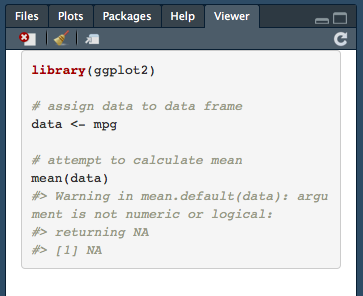
\includegraphics[width=0.5\linewidth]{images/reprex} \end{center}

It will also be available on your clipboard so that you can copy and
paste it into Slack or another venue that accepts Markdown syntax (like
GitHub). If your reprex contains image output, such as a plot or a map,
it will be automatically uploaded to imgur and a link will be embedded
in your Markdown syntax. For example, say we had a question about the
following code:

\begin{Shaded}
\begin{Highlighting}[]
\KeywordTok{library}\NormalTok{(ggplot2)}

\CommentTok{# assign data to data frame}
\NormalTok{data <-}\StringTok{ }\NormalTok{mpg}

\CommentTok{# plot highway mpg}
\KeywordTok{ggplot}\NormalTok{(}\DataTypeTok{data =}\NormalTok{ data, }\DataTypeTok{mapping =} \KeywordTok{aes}\NormalTok{(}\DataTypeTok{x =}\NormalTok{ hwy)) }\OperatorTok{+}\StringTok{ }
\StringTok{  }\KeywordTok{geom_histogram}\NormalTok{()}
\end{Highlighting}
\end{Shaded}

Once we copy the above code and render it using \texttt{reprex()}, it
will return the following output:

\begin{Shaded}
\begin{Highlighting}[]
\KeywordTok{library}\NormalTok{(ggplot2)}

\CommentTok{# assign data to data frame}
\NormalTok{data <-}\StringTok{ }\NormalTok{mpg}

\CommentTok{# plot highway mpg}
\KeywordTok{ggplot}\NormalTok{(}\DataTypeTok{data =}\NormalTok{ data, }\DataTypeTok{mapping =} \KeywordTok{aes}\NormalTok{(}\DataTypeTok{x =}\NormalTok{ hwy)) }\OperatorTok{+}\StringTok{ }
\StringTok{  }\KeywordTok{geom_histogram}\NormalTok{()}
\CommentTok{#> `stat_bin()` using `bins = 30`. Pick better value with `binwidth`.}

\OperatorTok{!}\NormalTok{[](https}\OperatorTok{:}\ErrorTok{//}\NormalTok{i.imgur.com}\OperatorTok{/}\NormalTok{8hiC7od.png)}
\end{Highlighting}
\end{Shaded}

The \texttt{!{[}{]}(hyperlink)} syntax will allow an image of your plot
to appear below the code.

The \href{http://reprex.tidyverse.org}{\texttt{reprex} package website}
has some great resources, including a
\href{http://reprex.tidyverse.org}{basic overview}, some
\href{http://reprex.tidyverse.org/articles/reprex-dos-and-donts.html}{reprex
do's and don'ts}, and a
\href{http://reprex.tidyverse.org/articles/articles/magic-reprex.html}{detailed
article} introducing the package's functionality.

\subsubsection{ArcGIS}\label{arcgis}

Creating a reprex in ArcGIS is not as straightforward since there is not
a dedicated tool for doing so like there is in \texttt{R}. Reprex
creation is complicated by the fact that many steps you will be taking
are manual. Nevertheless, it is possible to create a repex. Follow these
steps:

\begin{enumerate}
\def\labelenumi{\arabic{enumi}.}
\tightlist
\item
  In a new map document, load the minimum number of shapefiles needed to
  illustrate the issue you are having. Note where the shapefiles are
  available (in the course data release?) and what their names are.
\item
  Note what the coordinate system of the data frame is set to.
\item
  Provide notes for each step that gets you to your question or error.
\item
  Take a \href{https://www.take-a-screenshot.org}{screenshot} of the
  error or the window you have a question about.
\end{enumerate}

For example, a reprex of a question in ArcGIS could look like the
following:

\begin{verbatim}
1. I have a single map shapefile open in a new map document. The shapefile is the St. Louis census tracts shapefile from the example data in the course data release.
2. The coordinate system is Missouri State Plane East (Feet)
3. When I right click on the shapefile, I click on Properties and then the Symbology tab
4. Attached is a screenshot of what the symbology tab looks like for these data.
\end{verbatim}

\subsubsection{LaTeX}\label{latex}

Like ArcGIS, there is no specific tool for creating a reprex using
LaTeX. The LaTeX community does have, however, a long tradition of
creating ``minimal working examples'', which are similar to reprexs.
Follow these general steps:

\begin{enumerate}
\def\labelenumi{\arabic{enumi}.}
\tightlist
\item
  Create a new LaTeX project. Use the
  \texttt{\textbackslash{}documentclass\{article\}} if you are using
  something different.
\item
  Only include packages in the preamble that are \textbf{directly}
  related to the question or issue you have.
\item
  Skip creating a title block
\item
  Provide just enough body text in your LaTeX document to illustrate the
  issue.
\end{enumerate}

A repex for LaTeX might look something like this:

\begin{Shaded}
\begin{Highlighting}[]
\BuiltInTok{\textbackslash{}documentclass}\NormalTok{\{}\ExtensionTok{article}\NormalTok{\}}

\KeywordTok{\textbackslash{}begin}\NormalTok{\{}\ExtensionTok{document}\NormalTok{\}}

\FunctionTok{\textbackslash{}textbold}\NormalTok{\{Foo bar.\} Spam and eggs.}

\KeywordTok{\textbackslash{}end}\NormalTok{\{}\ExtensionTok{document}\NormalTok{\}}
\end{Highlighting}
\end{Shaded}

Also provide a written description of what is wrong (such as ``the text
is not being rendered as bold'') and, if helpful, a
\href{https://www.take-a-screenshot.org}{screenshot} of your output.
There is a great
\href{https://tex.meta.stackexchange.com/questions/228/ive-just-been-asked-to-write-a-minimal-example-what-is-that}{overview
on Stack Exchange} of how to write a reprex for LaTeX. If you are using
ShareLaTeX, also take a look at the error log and take a
\href{https://www.take-a-screenshot.org}{screenshot} of the relevant
error message. If you are using another LaTeX application, provide the
text of your error message instead.

\subsubsection{Other Tools}\label{other-tools}

For other tools we learn, such as Markdown and GitHub, you want to
follow the spirit of the reprex file. Try to recreate your issue outside
of the context of your assignment (this may not be possible for GitHub),
and provide a detailed walk-through of the steps that you took to get
where you are. For Markdown syntax, provide an example of the syntax you
are using that recreates the issue or question. For GitHub, provide a
\href{https://www.take-a-screenshot.org}{screenshot} of the relevant
error message.

\subsection{\texorpdfstring{``I don't think I can make a
reprex!''}{I don't think I can make a reprex!}}\label{i-dont-think-i-can-make-a-reprex}

I am 99\% sure that you can! In nearly every situation I have seen
students in, creating a reprex is possible. Even if the error is
idiosyncratic to your computer or your data, you can absolutely clarify
the context within which the error appears and minimize the amount of
data, code, and other information in your \texttt{R} code or your map
document. For the less than 1\% of scenarios where a reprex is not
possible, the process of writing a question, clarifying the context and
steps you took to get there, and producing an example of the error will
still make it easier for me to help you.

\subsection{\texorpdfstring{``Isn't this a lot of
work?''}{Isn't this a lot of work?}}\label{isnt-this-a-lot-of-work}

Well, yes, it does require some extra effort. This effort is almost
always worth it, however. In some cases, the time it takes you to
produce the repex leads you to the answer on your own, which is part of
the problem solving process that this class is designed to foster. Even
when this does not happen, making reprex informed inquries is a
technique that you will be able to take with you at the end of the
semester. Even if you are not working in a technical setting, being able
to structure clear, concise questions about a process is a valuable
skill!

Finally, creating a reprex saves you time in the long run. When I get
vague questions, it often takes some experimenting on my part to
reproduce the error. If you send me a question with a reproducible
error, you cut out that experimentation time on my end and I can get
right to answering your question. Likewise, students often come to
office hours without an example of their issue ready to go and hope that
I can conjure in my mind the scenario they are describing. Despite my
best efforts, I am usually unable to do so and ask students to reproduce
the error during office hours. If you come to office hours with a
reprex, we can get to answering your question right away!

\section{Where to Seek Help}\label{where-to-seek-help}

Once you have tried \protect\hyperlink{helping-yourself}{Helping
Yourself} and have gone through the steps outlined in
\protect\hyperlink{how-to-seek-help}{How to Seek Help} (i.e.~made a
reprex), it is time to ask your question. There are a number of
different places that you can pose questions. The sections below outline
these and suggest some ways to make your question most effective.

\subsection{Internal Venues}\label{internal-venues}

Within the confines of the course, the two best places to ask questions
are on Slack and during office hours. When asking a question on Slack,
please consider doing so in a public channel. This helps others learn
from the question that you have. The only course-related questions that
are not appropriate for Slack are those that reference specific parts of
a problem set or the final project. However, if you are creating
reproducible examples, your questions should not be that specific even
if they ultimately are about a homework assignment. If you are not sure
whether the question is appropirate or not for a public channel, or just
would prefer not to ask your question out in the open, feel free to send
me a
\href{https://get.slack.help/hc/en-us/articles/212281468-Direct-messages-and-group-DMs}{direct
message on Slack}.

When you pose a question on Slack, it should contain three or four
pieces of information:

\begin{enumerate}
\def\labelenumi{\arabic{enumi}.}
\tightlist
\item
  The question itself - what are you hoping to get help with?
\item
  A reproducible example - give as many details as you need to clearly
  illustrate the question
\item
  A \href{https://www.take-a-screenshot.org}{screenshot} or image output
  that illustrates your reprex
\item
  What you've tried - lay out the steps you took to quickly (``I've
  checked the spelling, gone through the Lecture 03 documents, looked at
  the \texttt{dplyr} website, and have done a quick Google search.'')
\end{enumerate}

Post your reprex as a
\href{https://get.slack.help/hc/en-us/articles/204145658-Create-a-snippet}{snippet}
in Slack by:

\begin{enumerate}
\def\labelenumi{\arabic{enumi}.}
\tightlist
\item
  Clicking the plus sign on the left side of the message box
\item
  Selecting \textbf{Code or text snippet}
\item
  Filling out the pop-up window
\end{enumerate}

If you are posting a reprex from \texttt{R}, remove the three backticks
and the letter \texttt{r} from the first line as well as the three
backticks from the bottom line. If you are including an image hyperlink
created by the \texttt{reprex} package, remove that from the code
snippet and paste it into Slack separately. A good question on Slack
should look like this:

\begin{center}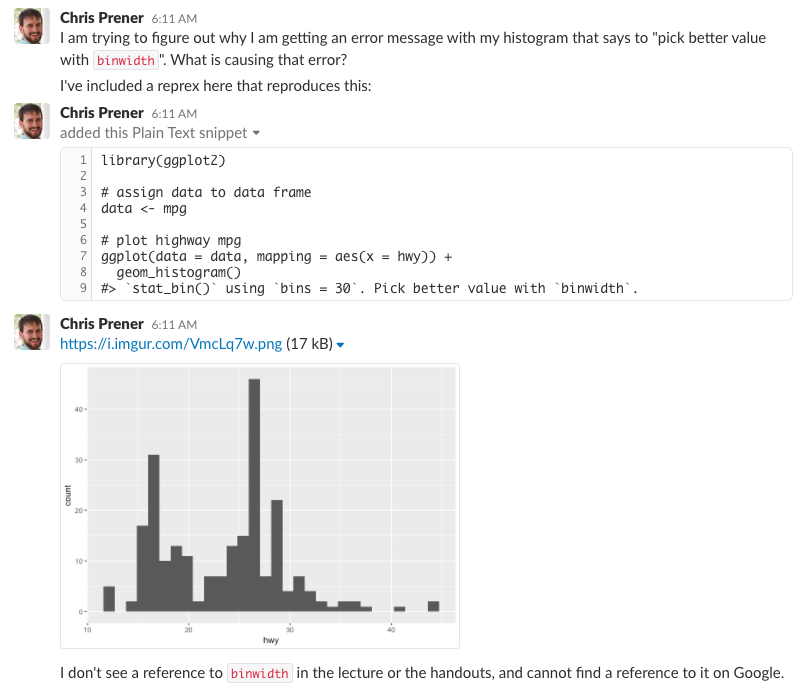
\includegraphics[width=0.9\linewidth]{images/slackQuestion} \end{center}

This same general process holds for asking questions in person - come
ready with a solid question, a reproducible example, and be ready to
pull it up on your computer or a lab computer.

\subsection{External Venues}\label{external-venues}

There are two good places to ask questions external to the course as
well. For questions related to RStudio, R Markdown, and the
\href{http://tidyverse.org}{tidyverse}, RStudio maintains a web forumn
called \href{https://community.rstudio.com}{RStudio Community}. If you
are posting there, you can use \texttt{reprex()} to generate Markdown
formatted reprexs.

Another place to post questions in on one of the relevant
\href{https://stackexchange.com}{Stack Exchange} communities:

\begin{itemize}
\tightlist
\item
  \href{https://stackoverflow.com}{Stack Overflow} for \texttt{R}, Git,
  and GitHub - post using tags like \texttt{{[}r{]}},
  \texttt{{[}ggplot2{]}}, \texttt{{[}dplyr{]}}, \texttt{{[}git{]}},
  \texttt{{[}github{]}}, etc.
\item
  \href{https://gis.stackexchange.com}{Geographic Information Systems}
  for GIS - post using the \texttt{{[}arcgis-desktop{]}} tag
\item
  \href{https://tex.stackexchange.com}{TeX} for LaTeX
\end{itemize}

Before you post, search thoroughly to make sure that your question has
not already been answered. Stack Exchange has strong norms about how to
post appropriately. You can descriptions of what makes a good post
\href{https://codereview.stackexchange.com/help/how-to-ask}{here} and
\href{https://stackoverflow.com/help/how-to-ask}{here}. You can also
find a description of
\href{https://stackoverflow.com/help/dont-ask}{what not to ask}. If you
are going to post on Stack Overflow, the \texttt{reprex()} function can
be modified to produce well-formatted output specific to that site by
adding the \texttt{venue} argument, as in
\texttt{reprex(venue\ =\ "so")}.

Of the two sites, I find \href{https://community.rstudio.com}{RStudio
Community} to be a friendlier place that is more relaxed thatn Stack
Overflow and its cousins. However, Stack Exchange communities have much
larger user bases to draw from.

\bibliography{book.bib,packages.bib}


\end{document}
